\documentclass[12pt]{report} 
\usepackage[utf8]{inputenc}
\usepackage[vietnamese]{babel}
\usepackage{amsmath}  % Lệnh hỗ trợ viết hệ phương trình
\usepackage{amssymb}  % Lệnh hỗ trợ viết ký hiệu số thực R
\usepackage{mathptmx} 
\usepackage{type1cm}
\usepackage{graphicx} % chèn hình ảnh
\begin{document}
% Thiết lập cỡ chữ 14pt và khoảng cách dòng 18pt
\fontsize{14pt}{18pt}\selectfont
\begin{center}
    \textbf{\Large LỜI CẢM ƠN}
\end{center}

\vspace{0.5cm}

\noindent Trong quá trình thực hiện dự án với dự án: \textit{"Phương pháp đặt ẩn phụ tỉ lệ trong giải hệ phương trình và bài toán cực trị đại số"}, em đã nhận được sự hướng dẫn, giúp đỡ và động viên quý báu từ quý thầy cô cùng bạn bè.

\vspace{0.3cm}
\noindent Trước hết, em xin bày tỏ lòng biết ơn sâu sắc đến thầy Nguyễn Đăng Minh Phúc - giảng viên trực tiếp hướng dẫn đã tận tình chỉ bảo, định hướng và góp ý cho em trong suốt quá trình thực hiện. Những kiến thức chuyên môn trong nghiên cứu cùng sự tận tâm của thầy đã giúp em vượt qua nhiều khó khăn để hoàn thành tốt dự án.

\vspace{0.3cm}
\noindent Em xin chân thành cảm ơn quý thầy cô trong Khoa Toán đã truyền đạt cho em những kiến thức nền tảng quý giá và tạo điều kiện thuận lợi nhất cho em trong suốt quá trình học tập, nghiên cứu tại trường.

\vspace{0.3cm}
\noindent Bên cạnh đó, em xin gửi lời cảm ơn đến các bạn sinh viên lớp/Khoa Toán đã luôn đồng hành, chia sẻ tài liệu, đóng góp ý kiến và động viên em trong suốt thời gian qua.

\vspace{0.3cm}
\noindent Do thời gian nghiên cứu và năng lực bản thân còn hạn chế, dự án khó tránh khỏi những thiếu sót nhất định. Em rất mong nhận được những lời nhận xét và góp ý quý báu từ quý thầy cô và các bạn để dự án được hoàn thiện hơn.

\vspace{0.3cm}
\noindent Em xin chân thành cảm ơn!

\vspace{1cm}
% Đẩy khối thông tin ngày tháng và ký tên sang bên phải
\begin{flushright}
    \textit{Thành phố Huế, tháng 9 năm 2026} \\
    \textbf{Sinh viên thực hiện} \\
    Trương Thị Như Ngọc
\end{flushright}
\newpage
\begin{center}
    \textbf{\Large MỤC LỤC}
\end{center}

\vspace{0.5cm}


\noindent \textbf{LỜI CẢM ƠN} \dotfill 1 \\
\noindent \textbf{MỞ ĐẦU} \dotfill 3 \\
\noindent \textbf{CHƯƠNG 1 CƠ SỞ LÍ THUYẾT CỦA PHƯƠNG PHÁP ĐẶT ẨN PHỤ TỈ LỆ} \dotfill 5 \\
\hspace*{0.5cm} 1.1. Quan hệ tỉ lệ giữa các biến số thực \dotfill 5 \\
\hspace*{0.5cm} 1.2. Trường hợp đặt một ẩn theo một ẩn \dotfill 5 \\
\hspace*{0.5cm} 1.3. Trường hợp đặt nhiều ẩn theo một ẩn \dotfill 6 \\
\hspace*{0.5cm} 1.4. Điều kiện áp dụng phương pháp đặt ẩn phụ tỉ lệ \dotfill 10 \\
\noindent \textbf{CHƯƠNG 2 ỨNG DỤNG TRONG GIẢI HỆ PHƯƠNG TRÌNH} \dotfill 11 \\
\noindent \textbf{CHƯƠNG 3. ỨNG DỤNG TRONG BÀI TOÁN TÌM GIÁ TRỊ LỚN NHẤT, GIÁ TRỊ NHỎ NHẤT} \dotfill 30 \\
\noindent \textbf{KẾT LUẬN} \dotfill 44 \\
\noindent \textbf{TÀI LIỆU THAM KHẢO} \dotfill 46
\newpage
\begin{center}
    \textbf{\Large MỞ ĐẦU}
\end{center}

\vspace{0.5cm}

\noindent Trong chương trình toán học phổ thông và đại học, hệ phương trình đại số và các bài toán tìm giá trị lớn nhất, giá trị nhỏ nhất của biểu thức đại số luôn giữ vai trò quan trọng. Đây không chỉ là những nội dung cơ bản của đại số sơ cấp mà còn có nhiều ứng dụng trong các lĩnh vực như vật lí, kĩ thuật, kinh tế và khoa học tính toán. Vì vậy, việc tìm kiếm các phương pháp giải hiệu quả, có tính định hướng và khả năng khái quát cao luôn là một vấn đề được quan tâm. Trong số các phương pháp thường được sử dụng, phương pháp đặt ẩn phụ là một công cụ quen thuộc và có hiệu quả trong việc đơn giản hóa bài toán. Đặc biệt, đối với các hệ phương trình đồng bậc, các biểu thức thuần nhất hoặc những bài toán xuất hiện quan hệ tỉ lệ giữa các biến, việc sử dụng phép đặt ẩn phụ tỉ lệ thường giúp giảm số lượng biến, làm xuất hiện các cấu trúc đại số quen thuộc và tạo thuận lợi cho quá trình biến đổi.

\vspace{0.3cm}
\noindent Không chỉ được ứng dụng trong giải hệ phương trình, phương pháp đặt ẩn phụ tỉ lệ còn hiệu quả trong các bài toán cực trị đại số. Việc đưa các biến về quan hệ tỉ lệ thích hợp giúp biểu thức cần khảo sát trở thành hàm của một biến hoặc xuất hiện các dạng bất đẳng thức quen thuộc, từ đó tạo điều kiện thuận lợi để áp dụng các công cụ như đạo hàm, bất đẳng thức cổ điển hoặc tính đơn điệu của hàm số.

\vspace{0.3cm}
\noindent Xuất phát từ những lí do trên, em chọn dự án \textit{"Phương pháp đặt ẩn phụ tỉ lệ trong giải hệ phương trình và bài toán cực trị đại số."}

\vspace{0.3cm}
\noindent Mục tiêu của dự án là hệ thống hóa cơ sở lí thuyết của phương pháp đặt ẩn phụ tỉ lệ, làm rõ điều kiện áp dụng và cách khai thác quan hệ tỉ lệ giữa các biến số thực. Trên cơ sở đó, dự án vận dụng phương pháp để giải một số hệ phương trình đại số và bài toán tìm giá trị lớn nhất, giá trị nhỏ nhất của biểu thức đại số nhằm làm nổi bật tính hiệu quả và tính linh hoạt của phương pháp.

\vspace{0.3cm}
\noindent Phạm vi nghiên cứu của dự án chủ yếu tập trung vào các hệ phương trình đại số hữu hạn và các bài toán cực trị trong phạm vi đại số sơ cấp trên tập số thực. Các ví dụ và bài toán minh họa được lựa chọn chủ yếu từ chương trình toán phổ thông nâng cao và một số tài liệu tham khảo chuyên đề.

\vspace{0.3cm}
\noindent Nội dung của dự án gồm ba chương:

\vspace{0.2cm}
\noindent $\bullet$ \textbf{Chương 1. Cơ sở lí thuyết của phương pháp đặt ẩn phụ tỉ lệ} \\
Trình bày các quan hệ tỉ lệ giữa các biến số thực, điều kiện áp dụng phương pháp và các trường hợp đặc biệt cần lưu ý khi sử dụng phép đặt ẩn phụ tỉ lệ.

\vspace{0.2cm}
\noindent $\bullet$ \textbf{Chương 2. Ứng dụng trong giải hệ phương trình đại số} \\
Vận dụng phương pháp đặt ẩn phụ tỉ lệ để giải một số hệ phương trình hai ẩn và ba ẩn thông qua các ví dụ minh họa tiêu biểu.

\vspace{0.2cm}
\noindent $\bullet$ \textbf{Chương 3. Ứng dụng trong bài toán tìm giá trị lớn nhất, giá trị nhỏ nhất} \\
Trình bày việc áp dụng phương pháp vào các bài toán cực trị đại số, kết hợp với các công cụ như đạo hàm và bất đẳng thức để tìm giá trị lớn nhất, giá trị nhỏ nhất của biểu thức.

\newpage
\noindent \textbf{CHƯƠNG 1. CƠ SỞ LÍ THUYẾT CỦA PHƯƠNG PHÁP ĐẶT ẨN PHỤ TỈ LỆ}

\vspace{0.3cm}
\noindent \textbf{1.1. Quan hệ tỉ lệ giữa các biến số thực}

\vspace{0.2cm}
Trong nhiều bài toán đại số, đặc biệt là các hệ phương trình đồng bậc và các bài toán tìm giá trị lớn nhất, giá trị nhỏ nhất, giữa các biến thường tồn tại những quan hệ tỉ lệ. Việc khai thác các quan hệ này thông qua phương pháp đặt ẩn phụ giúp giảm số lượng biến số, làm xuất hiện các cấu trúc quen thuộc và đơn giản hóa bài toán.

Một dạng đặt ẩn phụ tỉ lệ thường gặp là:
\[ %Đưa toàn bộ công thức toán học nằm ở giữa hai dấu này ra chính giữa một dòng riêng biệt
\begin{cases} % Lệnh bắt đầu tạo dấu ngoặc nhọn 
y = kx
\\ %lệnh xuống dòng 
z = lx 
\end{cases}
\]
với $k, l \in \mathbb{R}$. %Khi muốn viết các ký hiệu toán học nhỏ nằm ngay trong dòng chữ, kẹp chúng giữa hai dấu $

Tuy nhiên, để phép đặt ẩn phụ tỉ lệ có cơ sở và không làm mất nghiệm của bài toán, cần xét các điều kiện tồn tại của các quan hệ trên. Trong mục này, ta trình bày một số cơ sở cho việc áp dụng phương pháp đặt ẩn phụ tỉ lệ.

\vspace{0.4cm}
\noindent \textbf{1.2. Trường hợp đặt một ẩn theo một ẩn}

\vspace{0.2cm}
\noindent \textbf{Mệnh đề 1.2.1.} \textit{Cho $x, y, k$ là ba số thuộc tập hợp số thực $\mathbb{R}$, giả sử ta biểu thị $x$ qua $y$ thông qua phép toán nhân với $k$, tức là $x = ky$ (1) khi đó, ta xét các khả năng sau (các khả năng sau là độc lập với nhau):}

(1.i) $k \neq 0, x \neq 0, y \neq 0$, lúc đó lúc đó quan hệ tỉ lệ $x = ky$ được xác định.

(1.ii) $k \neq 0$, bộ số $(x; y)$ có một số bằng 0, một số khác 0 thì ta không biểu thị được (1).

(1.iii) $k = 0$, lúc đó $x = 0, \forall y \in \mathbb{R}$

(1.iv) $k \in \mathbb{R}, (x; y) = (0; 0)$ lúc đó (1) luôn đúng.

\vspace{0.3cm}
\noindent \textbf{Chứng minh.} Giả sử ta có $x = ky$ (1) với:
\begin{itemize} % danh sách các dấu chấm đầu dòng
      \item Giả thiết $k \neq 0$, bộ số $(x; y)$ có một số bằng 0, một số khác 0, xét 2 trường hợp sau:
    
    \textbf{TH1.} Nếu $\begin{cases} x = 0 \\ y \neq 0 \end{cases}$ thì từ (1), ta có: $0 = ky$, mà $k \neq 0, y \neq 0$ nên $ky \neq 0$ (mâu thuẫn), do đó (1) không biểu thị được.
    
    \textbf{TH2.} Nếu $y = 0, x \neq 0$ thì từ (1), ta có: $x = k \cdot 0 \Leftrightarrow x = 0$, mâu thuẫn với giả thiết $x \neq 0$, do đó (1) không biểu thị được.
    
    Từ 2 trường hợp trên, rõ ràng (1) không biểu thị được, do đó (1.ii) được chứng minh.
    
    \item Giả thiết $k = 0$, lúc đó thay $k = 0$ vào (1) ta được $x = 0 \cdot y = 0, \forall y \in \mathbb{R}$, do đó (1.iii) được chứng minh.
    
    \item Giả thiết $k \in \mathbb{R}, (x; y) = (0; 0)$, lúc đó thay $(x; y) = (0; 0)$ vào (1) ta được $0 = k \cdot 0 = 0$, luôn đúng với mọi $k \in \mathbb{R}$, do đó (1.iv) được chứng minh.
\end{itemize}

\vspace{0.4cm}
\noindent \textbf{1.3. Trường hợp đặt nhiều ẩn theo một ẩn}

\vspace{0.2cm}
\noindent \textbf{Mệnh đề 1.3.1.} \textit{Cho $x, y, z, k, l$ là năm số thuộc tập hợp số thực $\mathbb{R}$, giả sử ta biểu thị $y$ qua $x$ thông qua phép toán nhân với $k$ và $z$ qua $x$ thông qua phép toán nhân với $l$ tức là $\begin{cases} y = kx \\ z = lx \end{cases}$ (2) khi đó, ta xét các khả năng sau (các khả năng sau là độc lập với nhau):}

\vspace{0.3cm}
\noindent (2.i) $\begin{cases} k \neq 0 \\ l \neq 0 \end{cases}, x \neq 0, y \neq 0, z \neq 0$, lúc đó quan hệ tỉ lệ $\begin{cases} y = kx \\ z = lx \end{cases}$ được xác định.

\vspace{0.3cm}
\noindent (2.ii) $\begin{cases} k \neq 0 \\ l \neq 0 \end{cases}$, bộ số $(x; y; z)$ có một số bằng 0, hai số còn lại khác 0 hoặc hai số bằng 0, một số còn lại khác 0 thì ta không biểu thị được (2).

\vspace{0.3cm}
\noindent (2.iii) $k = l = 0$, lúc đó $y = z = 0, \forall x \in \mathbb{R}$.

\vspace{0.3cm}
\noindent (2.iv) $\begin{cases} k \in \mathbb{R} \\ l \in \mathbb{R} \end{cases}, (x; y; z) = (0; 0; 0)$ lúc đó (2) luôn đúng.

\noindent (2.v) Nếu một trong hai số $k$ hoặc $l$ có một số bằng 0, số còn lại khác 0 thì bộ số $(x; y; z)$ có một số bằng 0, hai số còn lại được biểu thị với nhau thông qua phép toán nhân với hằng số $k$ hoặc $l$ khác 0.

\vspace{0.4cm}
\noindent \textbf{Chứng minh.} Giả sử ta có $\begin{cases} y = kx \\ z = lx \end{cases}$ (2) với:

\vspace{0.3cm}
\noindent $\bullet$ Giả thiết $\begin{cases} k \neq 0 \\ l \neq 0 \end{cases}, x \neq 0, y \neq 0, z \neq 0$, rõ ràng phép toán nhân ở (2) được xét trong tập hợp số thực $\mathbb{R}$ luôn tồn tại, tức luôn biểu thị được (2), do đó (2.i) được chứng minh.

\vspace{0.3cm}
\noindent $\bullet$ Giả thiết $\begin{cases} k \neq 0 \\ l \neq 0 \end{cases}$, bộ số $(x; y; z)$ có một số bằng 0, hai số còn lại khác 0 hoặc hai số bằng 0, một số còn lại khác 0, xét 2 trường hợp sau:

\vspace{0.3cm}
\noindent \textbf{TH1.} Có một số bằng 0, hai số còn lại khác 0.

\vspace{0.2cm}
\noindent + Nếu $x = 0, y \neq 0, z \neq 0$ thì từ (2), ta có $\begin{cases} y = k \cdot 0 = 0 \\ z = l \cdot 0 = 0 \end{cases}$, mâu thuẫn với giả thiết $\begin{cases} y \neq 0 \\ z \neq 0 \end{cases}$ do đó (2) không biểu thị được.

\vspace{0.2cm}
\noindent + Nếu $x \neq 0, y = 0, z \neq 0$ thì từ (2), ta có $\begin{cases} 0 = k \cdot x = 0 \\ z = l \cdot x \end{cases}$, từ đây ta thấy $k = 0$ hoặc $x = 0$, mâu thuẫn với giả thiết $x \neq 0, k \neq 0$ do đó (2) không biểu thị được.

\vspace{0.2cm}
\noindent + Nếu $x \neq 0, y \neq 0, z = 0$ thì từ (2), ta có $\begin{cases} y = kx \\ 0 = lx \end{cases} \Leftrightarrow \begin{cases} y = kx \\ l = 0 \end{cases}$, mâu thuẫn với giả thiết $l \neq 0$, do đó (2) không biểu thị được.

\vspace{0.3cm}
\noindent \textbf{TH2.} Có hai số bằng 0, một số còn lại khác 0.

\vspace{0.2cm}
\noindent + Nếu $x \neq 0, y = 0, z = 0$ thì từ (2), ta có $\begin{cases} 0 = kx \\ 0 = lx \end{cases} \Leftrightarrow \begin{cases} k = 0 \\ l = 0 \end{cases}$, mâu thuẫn với giả thiết $\begin{cases} k \neq 0 \\ l \neq 0 \end{cases}$, do đó (2) không biểu thị được.

\vspace{0.2cm}
\noindent + Nếu $x = 0, y \neq 0, z = 0$ thì từ (2), ta có $\begin{cases} y = k \cdot 0 = 0 \\ 0 = l \cdot 0 = 0 \end{cases} \Leftrightarrow y = 0$, mâu thuẫn với giả thiết $y \neq 0$, do đó (2) không biểu thị được.

\noindent 
+ Nếu $x = 0, y = 0, z \neq 0$ thì từ (2), ta có $\begin{cases} 0 = k \cdot 0 = 0 \\ z = l \cdot 0 = 0 \end{cases} \Leftrightarrow z = 0$, mâu thuẫn với giả thiết $z \neq 0$, do đó (2) không biểu thị được.

\vspace{0.2cm}
\noindent Từ các khả năng trên, rõ ràng (2) không biểu thị được, do đó (2.ii) được chứng minh.

\vspace{0.3cm}
\noindent $\bullet$ Giả thiết $k = l = 0$, lúc đó thay vào (2) ta được $\begin{cases} y = 0 \cdot x = 0 \\ z = 0 \cdot x = 0 \end{cases}, \forall x \in \mathbb{R}$, do đó (2.iii) được chứng minh.

\vspace{0.3cm}
\noindent $\bullet$ Giả thiết $k \in \mathbb{R}, l \in \mathbb{R}, (x; y; z) = (0; 0; 0)$, lúc đó thay $(x; y; z) = (0; 0; 0)$ vào (2) ta được $\begin{cases} 0 = k \cdot 0 = 0 \\ 0 = l \cdot 0 = 0 \end{cases}$, luôn đúng với mọi $k, l \in \mathbb{R}$, do đó (2.iv) được chứng minh.

\vspace{0.3cm}
\noindent $\bullet$ Nếu một trong hai số $k$ hoặc $l$ có một số bằng 0, số còn lại khác 0, từ (2) ta xét:

\vspace{0.2cm}
\noindent \textbf{TH1.} Nếu $\begin{cases} k = 0 \\ l \neq 0 \end{cases}$ thì $\begin{cases} y = 0 \cdot x = 0 \\ z = l \cdot x \end{cases}$, rõ ràng $y = 0, z$ và $x$ được biểu thị với nhau thông qua phép toán nhân với hằng số $l \neq 0$.

\vspace{0.2cm}
\noindent \textbf{TH2.} Nếu $\begin{cases} k \neq 0 \\ l = 0 \end{cases}$ thì $\begin{cases} y = k \cdot x \\ z = 0 \cdot x = 0 \end{cases}$, rõ ràng $z = 0, y$ và $x$ được biểu thị với nhau thông qua phép toán nhân với hằng số $k \neq 0$.

\vspace{0.2cm}
\noindent Do đó (2.v) được chứng minh.

\vspace{0.4cm}
\noindent \textit{\textbf{Lưu ý:} Trong quá trình giải toán, khi các biến của bài toán thỏa mãn điều kiện của Mệnh đề 1.2.1 hoặc Mệnh đề 1.3.1 thì việc đặt ẩn phụ tỉ lệ là có cơ sở. Tuy nhiên, cần xét riêng các trường hợp đặc biệt như:}

\vspace{0.2cm}
\noindent $\bullet$ một hoặc nhiều biến bằng 0;

\vspace{0.1cm}
\noindent $\bullet$ tham số tỉ lệ bằng 0;

\vspace{0.1cm}
\noindent $\bullet$ các trường hợp có thể làm mất nghiệm hoặc phát sinh nghiệm ngoại lai.

\vspace{0.2cm}
\noindent Việc xét đầy đủ các khả năng trên giúp phương pháp đặt ẩn phụ được áp dụng một cách chặt chẽ và hiệu quả.

\vspace{0.4cm}
\noindent \textbf{1.4. Điều kiện áp dụng phương pháp đặt ẩn phụ tỉ lệ}

\noindent Trong thực hành giải toán, \textit{phương pháp đặt ẩn phụ tỉ lệ thường được áp dụng} hiệu quả trong các trường hợp sau:

\vspace{0.2cm}
\noindent $\bullet$ Hệ phương trình đồng bậc;

\vspace{0.1cm}
\noindent $\bullet$ Các biểu thức có cùng bậc giữa các biến;

\vspace{0.1cm}
\noindent $\bullet$ Các biểu thức chứa tỉ số giữa các biến;

\vspace{0.1cm}
\noindent $\bullet$ Các bài toán cực trị có cấu trúc đối xứng hoặc thuần nhất.

\vspace{0.3cm}
\noindent Khi áp dụng phương pháp, cần chú ý:

\vspace{0.2cm}
\noindent $\bullet$ xét riêng các trường hợp biến bằng 0;

\vspace{0.1cm}
\noindent $\bullet$ tránh chia cho 0;

\vspace{0.1cm}
\noindent $\bullet$ kiểm tra đầy đủ điều kiện của các tham số tỉ lệ;

\vspace{0.1cm}
\noindent $\bullet$ đối chiếu nghiệm tìm được với điều kiện ban đầu của bài toán để tránh mất nghiệm hoặc nhận nghiệm ngoại lai.

\vspace{0.3cm}
\newpage
\noindent \textbf{CHƯƠNG 2. ỨNG DỤNG TRONG GIẢI HỆ PHƯƠNG TRÌNH}

\vspace{0.3cm}
\noindent Các bài toán trong mục này là các hệ phương trình hai ẩn hoặc ba ẩn được xét trên tập số thực $\mathbb{R}$.

\vspace{0.3cm}
\noindent \textbf{Phương pháp chung:} Dựa vào điều kiện của Mệnh đề 1.2.1 hoặc Mệnh đề 1.3.1 và đặc điểm của từng hệ phương trình, ta tiến hành đặt ẩn phụ tỉ lệ thích hợp. Sau khi thay các ẩn phụ vào hệ, thông qua các phép biến đổi tương đương, hệ phương trình được đưa về dạng chứa một hoặc nhiều ẩn phụ. Tiếp theo, sử dụng các phương pháp đại số quen thuộc như phép thế, phép cộng đại số hoặc phân tích nhân tử để quy về phương trình một ẩn phụ. Cuối cùng, đối chiếu với điều kiện của bài toán để tìm nghiệm của hệ phương trình ban đầu và kết luận.

\vspace{0.4cm}
\noindent \textbf{Bài toán 1.} \textit{Giải hệ phương trình:}
\[ (1^*)
\begin{cases}
2(y^2 - x^2) = \dfrac{14}{x} - \dfrac{13}{y} \quad (1.1) \\[10pt]
4(x^2 + y^2) = \dfrac{14}{x} + \dfrac{13}{y} \quad (1.2)
\end{cases}
\]

\begin{itemize}
    \item[\textbf{1.}] \textbf{Hướng giải (Vì sao đưa ra bài toán này):} 
    Ban đầu hệ phương trình chứa các phân thức cồng kềnh với ẩn nằm ở mẫu ($x, y$), tạo cảm giác phức tạp và phi tuyến, xây dựng bài toán này nhằm rèn luyện tư duy biến đổi sơ cấp: thực hiện \textbf{cộng và trừ vế theo vế} hai phương trình để cô lập và triệt tiêu các phân thức, từ đó chuyển hệ ban đầu thành hệ phương trình đồng bậc bậc ba ($x^3 + 3y^2x = 14$ và $y^3 + 3x^2y = 13$). Đây chính là bước đệm tự nhiên để gợi ý áp dụng phép đặt ẩn phụ tỉ lệ $x = ky$ ($k \neq 0$).

    \item[\textbf{2.}] \textbf{Cái hay của bài toán:} 
    Quan sát tổng - hiệu để "khử" ẩn độc lập một cách tinh tế. Sau khi đặt ẩn phụ, phương trình ẩn $k$ thu được có nghiệm đẹp ($k=2$), kết hợp với bước đánh giá tam thức bậc hai vô nghiệm giúp lời giải cực kỳ chặt chẽ, loại bỏ hoàn toàn bẫy sót nghiệm.
\end{itemize}
\vspace{0.2cm}
\noindent \textbf{Lời giải.} ĐK: $x \neq 0, y \neq 0$. Với ĐK này ta thực hiện biến đổi như sau:

\vspace{0.2cm}
\noindent Cộng theo vế PT(1.1) cho PT(1.2), ta được:
\[
6y^2 + 2x^2 = 2 \cdot \dfrac{14}{x} \overset{x \neq 0}{\Leftrightarrow} x^3 + 3y^2x = 14 \quad (1.3)
\]

\vspace{0.2cm}
\noindent Trừ theo vế PT(1.1) cho PT(1.2), ta được:
\[
-2y^2 - 6x^2 = -2 \cdot \dfrac{13}{y} \overset{y \neq 0}{\Leftrightarrow} y^3 + 3x^2y = 13 \quad (1.4)
\]

\vspace{0.2cm}
\noindent Từ hai phép biến đổi trên, ta thu được HPT tương đương với hệ PT($1^*$):
\[
\begin{cases}
x^3 + 3y^2x = 14 \quad (1.3) \\
y^3 + 3x^2y = 13 \quad (1.4)
\end{cases}
\]

\vspace{0.2cm}
\noindent Giả sử có $x = ky$, từ ĐK ta có $k \neq 0$, $k$ là ẩn số phụ, khi đó biến số thỏa mãn Mệnh đề 1.2.1 -- (1.i) nên ta có thể đặt $x = ky$, $k \neq 0$ thay vào PT(1.3) và PT(1.4) thu được hệ:
\[
\begin{cases}
k^3y^3 + 3y^3k = 14 \quad (1.5) \\
y^3 + 3k^2y^3 = 13 \quad (1.6)
\end{cases}
\]

\vspace{0.2cm}
\noindent $(1.6) \Leftrightarrow y^3(1 + 3k^2) = 13$
\noindent $\Leftrightarrow y^3 = \dfrac{13}{1 + 3k^2}$ (1.7) ($1 + 3k^2 > 0$)

\vspace{0.2cm}
\noindent Thay vào PT(1.5) ta được: $\dfrac{13k^3}{1 + 3k^2} + \dfrac{3.13k}{1 + 3k^2} = 14$

\vspace{0.2cm}
\noindent $\Leftrightarrow 13k^3 - 42k^2 + 39k - 14 = 0$

\vspace{0.2cm}
\noindent $\Leftrightarrow (k - 2)(13k^2 - 16k + 7) = 0$

\vspace{0.2cm}
\noindent $\Leftrightarrow (k - 2) \left[ \underbrace{13\left(k - \dfrac{8}{13}\right)^2 + \dfrac{27}{13}}_{P(k) > 0} \right] = 0 \Leftrightarrow k = 2$.

\vspace{0.3cm}
\noindent Với $k = 2$, kết hợp PT(1.7) và cách đặt $x = ky$, ta có: $\begin{cases} y^3 = \dfrac{13}{1 + 3.(2)^2} = 1 \\ x = 2y \end{cases} \Leftrightarrow \begin{cases} y = 1 \\ x = 2 \end{cases}$.

\vspace{0.2cm}
\noindent Kiểm tra lại bộ số $(x; y) = (2; 1)$ vào hệ PT($1^*$) thấy thỏa mãn.

\vspace{0.2cm}
\noindent \textbf{Kết luận:} $HPT(1^*)$ có nghiệm duy nhất $(x; y) = (2; 1)$.

\vspace{0.3cm}
\noindent \textbf{Nhận xét.}

\vspace{0.1cm}
\noindent Điểm mấu chốt của bài toán là sau khi cộng và trừ hai phương trình, hệ xuất hiện các biểu thức
\[
x^3 + 3xy^2, \quad y^3 + 3x^2y
\]
là các biểu thức đồng bậc bậc ba theo hai biến $x, y$. Điều này gợi ý tồn tại quan hệ tỉ lệ giữa hai biến, từ đó phép đặt
\[
x = ky
\]
giúp đưa hệ phương trình về phương trình chỉ chứa một ẩn phụ $k$.

\vspace{0.2cm}
\noindent Bài toán cho thấy phương pháp đặt ẩn phụ tỉ lệ đặc biệt hiệu quả đối với các hệ có cấu trúc đồng bậc và đối xứng không hoàn toàn.

\vspace{0.4cm}
\noindent \textbf{Bài toán 2.} \textit{Giải hệ phương trình}
\[
(2^*) \begin{cases}
4x^2y - 2xy^2 + 3y^3 - 2(x + y) = 0 \quad (2.1) \\
(2 - xy)(x^2 + y^2) = 4 - 2xy \quad (2.2)
\end{cases}
\]

\begin{itemize}
    \item[\textbf{1.}] \textbf{Hướng giải (Vì sao đưa ra bài toán này):} 
    Phương trình thứ hai thoạt nhìn rất cồng kềnh nhưng thực chất ẩn chứa cấu trúc nhân tử chung. Bài toán được đưa ra nhằm kiểm tra kỹ năng phân tích đa thức thành nhân tử để "chia để trị". Bằng cách biến đổi phương trình thứ hai thành $(2-xy)(x^2+y^2-2) = 0$, hệ được tách thành hai nhánh độc lập ($xy=2$ hoặc $x^2+y^2=2$). Kết hợp nhánh thuần nhất $x^2+y^2=2$ với phương trình thứ nhất qua phép đặt ẩn phụ tỉ lệ $x = ky$, ta giải quyết trọn vẹn bài toán.

    \item[\textbf{2.}] \textbf{Cái hay của bài toán:} 
    Sự kết hợp giữa phương pháp phân tích nhân tử (để tách nhánh) và phương pháp đặt ẩn phụ tỉ lệ (trên nhánh thuần nhất). Bài toán rèn luyện tư duy phân loại trường hợp linh hoạt, tránh được sự lúng túng khi đối mặt với hệ phương trình bậc cao.
\end{itemize}
\vspace{0.2cm}
\noindent \textbf{Lời giải.} Tập xác định $D = \mathbb{R}$, ta có PT:

\vspace{0.2cm}
\noindent $(2.2) \Leftrightarrow (2 - xy)(x^2 + y^2 - 2) = 0$
\[
\Leftrightarrow \left[ 
\begin{aligned}
&xy = 2 \quad (2.2.1) \\
&x^2 + y^2 = 2 \quad (2.2.2)
\end{aligned} 
\right.
\]

\vspace{0.2cm}
\noindent Ta xét hai trường hợp sau:

\noindent \textbf{TH1.} Xét PT $xy = 2$ (2.2.1). Dễ thấy $x = 0$ hoặc $y = 0$ không thỏa mãn PT(2.2.1), do đó với $x \neq 0$, ta có PT $(2.2.1) \Leftrightarrow y = \dfrac{2}{x}$, thay vào PT(2.1), ta nhận được:
\[
4x^2 \cdot \dfrac{2}{x} - 2x \left(\dfrac{2}{x}\right)^2 + 3\left(\dfrac{2}{x}\right)^3 - 2\left(x + \dfrac{2}{x}\right) = 0
\]
\[
\overset{x \neq 0}{\Leftrightarrow} 6x - \dfrac{12}{x} + \dfrac{24}{x^3} = 0 \overset{x \neq 0}{\Leftrightarrow} 6x^4 - 12x^2 + 24 = 0
\]
\[
\Leftrightarrow 6(x^2 - 1)^2 + 18 = 0\text{, PT này vô nghiệm trên R.}
\]

\noindent Do đó, ở trường hợp 1 HPT($2^*$) vô nghiệm.

\noindent \textbf{TH2.} Xét PT $x^2 + y^2 = 2$ (2.2.2).

\noindent Dễ thấy $(x; y) = (0; 0)$ không thỏa mãn PT(2.2.2), giả sử có $x = ky$ và vì $(x; y) \neq (0; 0)$ nên $k \neq 0$, $k$ là ẩn số phụ, khi đó các biến số thỏa mãn MỆNH ĐỀ 1.2.1 -- (1.i), nên ta có thể đặt $x = ky$, $k \neq 0$ thay vào PT(2.2.2) và PT(2.1) thu được hệ:
\[
\begin{cases}
(ky)^2 + y^2 = 2 \\
4(ky)^2y - 2(ky)y^2 + 3y^3 - 2(ky + y) = 0
\end{cases}
\]
\[
\Leftrightarrow \begin{cases}
y^2 = \dfrac{2}{k^2 + 1}\text{, } (k^2 + 1 > 0) \hfill (2.3) \\
y[y^2(4k^2 - 2k + 3) - 2(k + 1)] = 0 \hfill (2.4)
\end{cases}
\]

\noindent Ta có PT:
\[
(2.4) \Leftrightarrow \left[ 
\begin{aligned}
&y = 0 \hfill (2.4.1) \\
&y^2(4k^2 - 2k + 3) = 2(k + 1) \hfill (2.4.2)
\end{aligned} 
\right.
\]

\noindent Ta xét các trường hợp sau:

\noindent \textbf{TH2.1.} Từ (2.4.1) ta có $y = 0 \overset{x=ky}{\implies} x = 0$, bộ số $(x; y) = (0; 0)$ không thỏa mãn hệ PT($2^*$).

\noindent \textbf{TH2.2.} Từ (2.3) ta có $y^2 = \dfrac{2}{k^2 + 1}$, thay vào PT(2.4.2) ta được:
\[
\dfrac{2}{k^2 + 1} \times (4k^2 - 2k + 3) = 2(k + 1)
\]
\[
\Leftrightarrow k^3 - 3k^2 + 3k - 2 = 0 \Leftrightarrow (k - 2) \left( \underbrace{\left(k - \dfrac{1}{2}\right)^2 + \dfrac{3}{4}}_{P(k) > 0} \right) = 0
\]
\[
\Leftrightarrow k = 2 \overset{x=ky}{\implies} x = 2y \quad (2.5).
\]
\noindent Thay $k = 2$ vào PT(2.3) ta được:
\[
y^2 = \dfrac{2}{2^2 + 1} = \dfrac{2}{5} \Leftrightarrow y = \pm \dfrac{\sqrt{10}}{5} \overset{(2.5)}{\implies} x = \pm \dfrac{2\sqrt{10}}{5}
\]

\noindent Thử lại 2 bộ số $\left( \dfrac{2\sqrt{10}}{5}; \dfrac{\sqrt{10}}{5} \right)$; $\left( \dfrac{-2\sqrt{10}}{5}; \dfrac{-\sqrt{10}}{5} \right)$ vào lại hệ PT(2) ta thấy thỏa mãn.

\vspace{0.2cm}
\noindent \textbf{Kết luận:} $HPT(2)$ có hai nghiệm là
\[
(x; y) \in \left\{ \left( \dfrac{2\sqrt{10}}{5}; \dfrac{\sqrt{10}}{5} \right); \left( \dfrac{-2\sqrt{10}}{5}; \dfrac{-\sqrt{10}}{5} \right) \right\}.
\]

\noindent \textbf{Nhận xét:} Trong bài toán này, phương trình thứ hai được phân tích thành tích thành nhân tử:
\[
(2 - xy)(x^2 + y^2 - 2) = 0,
\]
từ đó hệ được chia thành các trường hợp riêng biệt.

\noindent Ở trường hợp
\[
x^2 + y^2 = 2,
\]
biểu thức mang tính thuần nhất bậc hai nên phép đặt
\[
x = ky
\]
giúp đưa hệ về phương trình chỉ còn một ẩn phụ $k$.

\vspace{0.2cm}
\noindent Bài toán cho thấy khi áp dụng phương pháp đặt ẩn phụ tỉ lệ cần kết hợp linh hoạt với các phép phân tích nhân tử và xét trường hợp.

\vspace{0.4cm}
\noindent \textbf{Bài toán 3.} \textit{Giải hệ phương trình}
\[
(3^*): \begin{cases}
2x^2 - 5xy - y^2 = 1 \hfill (3.1) \\
y(\sqrt{xy - 2y^2} + \sqrt{4y^2 - xy}) = 1 \hfill (3.2)
\end{cases}
\]

\begin{itemize}
    \item[\textbf{1.}] \textbf{Hướng giải (Vì sao đưa ra bài toán này):} 
    Bài toán được thiết kế để khai thác triệt để \textbf{điều kiện xác định của căn thức}. Từ điều kiện $4y^2 \ge xy \ge 2y^2 > 0$, ta chặn ngay được tỉ số $2 \le \frac{x}{y} \le 4$. Do cả hai phương trình cùng bằng $1$, việc trừ vế theo vế và đặt $x = ky$ ($k \in [2, 4]$) sẽ đưa phương trình về một ẩn $k$ chứa tổng hai căn thức, tạo cơ sở vững chắc để tìm nghiệm chính xác.

    \item[\textbf{2.}] \textbf{Cái hay của bài toán:} 
    Sự giao thoa tuyệt vời giữa miền giá trị của ẩn phụ và kỹ thuật lượng liên hợp nâng cao. Miền xác định $[2, 4]$ giúp khoanh vùng chính xác nghiệm nguyên $k=3$, làm tiền đề cho việc nhân lượng liên hợp cô lập nhân tử một cách hoàn hảo và đẹp mắt.
\end{itemize}
\vspace{0.2cm}
\noindent \textbf{Lời giải.} ĐK: $\begin{cases} xy - 2y^2 \geq 0 \\ 4y^2 - xy \geq 0 \\ y > 0 \end{cases}$
\[
\Leftrightarrow 4y^2 \geq xy \geq 2y^2 > 0 \Leftrightarrow 4y \geq x \geq 2y > 0
\]

\noindent Trừ theo vế PT(3.1) cho PT(3.2) ta nhận được:
\[
2x^2 - 5xy - y^2 = y(\sqrt{xy - 2y^2} + \sqrt{4y^2 - xy}) \quad (3.3).
\]
\noindent Giả sử có $x = ky$, theo ĐK ta có $x > 0, y > 0$ thì $k > 0$, $k$ là ẩn số phụ, khi đó biến số thỏa mãn MỆNH ĐỀ 1.2.1 -- (1.i) nên ta có thể đặt $x = ky$, $k > 0$, thay vào PT(3.3) ta được:
\[
2(ky)^2 - 5k^2y - y^2 = y(\sqrt{ky^2 - 2y^2} + \sqrt{4y^2 - ky^2})
\]
\[
\Leftrightarrow y^2(2k^2 - 5k - 1 - \sqrt{4 - k} - \sqrt{k - 2}) = 0\text{, }
\]
\centerline{(với $y > 0, k \in [2; 4]$)}
\[
\overset{y > 0}{\implies} \underbrace{2k^2 - 5k - 1 - \sqrt{4 - k} - \sqrt{k - 2} = 0}_{f(k)} \quad (3.4)
\]
\[
\Leftrightarrow 2k^2 - 5k - 3 - (\sqrt{4 - k} - 1) - (\sqrt{k - 2} - 1) = 0
\]
\[
\Leftrightarrow (2k + 1)(k - 3) + \dfrac{k - 3}{1 + \sqrt{4 - k}} - \dfrac{k - 3}{\sqrt{k - 2} + 1} = 0
\]
\centerline{\Big(với $\begin{cases} 1 + \sqrt{4 - k} > 0 \\ 1 + \sqrt{k - 2} > 0 \end{cases}, \forall k \in [2; 4]$\Big)}
\[
\Leftrightarrow (k - 3) \left( 2k + 1 + \dfrac{1}{1 + \sqrt{4 - k}} - \dfrac{1}{\sqrt{k - 2} + 1} \right) = 0
\]
\[
\Leftrightarrow (k - 3) \left[ \underbrace{2k + \dfrac{1}{1 + \sqrt{4 - k}} - \dfrac{\sqrt{k - 2}}{\sqrt{k - 2} + 1}}_{P(k) > 0, \forall k \in [2; 4]} \right] = 0
\]
\[
\Leftrightarrow k = 3\text{ (thỏa mãn } k \in [2; 4]\text{).}
\]

\noindent Với $k = 3 \overset{x=ky}{\implies} x = 3y$, thay vào PT(3.1), kết hợp ĐKXĐ ta có:
\[
\begin{cases}
2(3y)^2 - 5.(3y).y - y^2 = 1 \\
y > 0
\end{cases}
\]
\[
\Leftrightarrow \begin{cases} 2y^2 = 1 \\ y > 0 \end{cases} \Leftrightarrow y = \dfrac{1}{\sqrt{2}} \overset{x=3y}{\implies} x = \dfrac{3}{\sqrt{2}}\text{.}
\]

\noindent Kiểm tra lại bộ số $(x; y) = \left(\dfrac{3}{\sqrt{2}}; \dfrac{1}{\sqrt{2}}\right)$ vào hệ PT(3) thấy thỏa mãn.

\vspace{0.2cm}
\noindent \textbf{Kết luận:} $HPT(3^*)$ có nghiệm duy nhất là $(x; y) = \left(\dfrac{3}{\sqrt{2}}; \dfrac{1}{\sqrt{2}}\right)$.

\vspace{0.3cm}
\noindent \textbf{Bình luận:} Để có hướng giải như trên, ta sử dụng máy tính Casio f(x) -- 580VNX để dò đoán số nghiệm, ta đặt vế trái PT(3.4) là f(k) với chức năng bảng TABLE ta tính 45 giá trị trong đoạn $[2; 4]$, thu được kết quả hiển thị trên màn hình như sau.

\begin{center}
    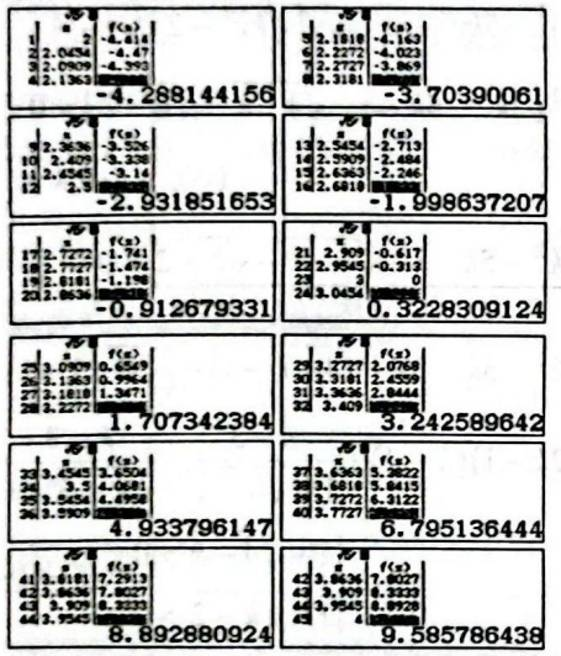
\includegraphics[width=0.65\textwidth]{bang_casio.jpg}
\end{center}

\vspace{0.3cm}
\noindent Quan sát bảng giá trị tính từ thứ tự 1 đến 22 và 24 đến 45, $f(x)$ (lưu ý vai trò ẩn $k$ bây giờ là ẩn $x$) chỉ đổi dấu từ "$-$" sang "$+$" một lần và tại thứ tự 23 của $x$ thì $f(x)$ nhận $x = 3$ làm nghiệm, vì vậy $f(k)=0$ chỉ có một nghiệm duy nhất trên $[2;4]$. 

\noindent Ngoài ra ta có thể giải tìm lại nghiệm bằng chức năng \textbf{SOLVE (SHIFT CALC)} khi đã biết chắc chắn có một nghiệm, về màn hình tính toán thông thường, nhập biểu thức $f(x)$ và ấn \textbf{SHIFT CALC}, chọn giá trị "\textit{khởi tạo}" có thể ngẫu nhiên trong $[2;4]$, chẳng hạn $x = 2.3$ ta tìm được nghiệm $x = 3$, tiếp tục tìm nghiệm còn lại ta chia $f(x)$ cho $(x - 3)$ ấn \textbf{SHIFT CALC} chờ máy giải thì kết quả màn hình hiển thị "\textit{không giải được}".

\vspace{0.4cm}
\begin{center}
    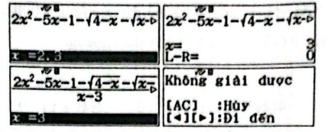
\includegraphics[width=0.7\textwidth]{anh2.png}
\end{center}

\vspace{0.3cm}
\noindent Ta thay $k_0 = 3$ vào mỗi căn thức thì được

\[
\begin{cases}
\sqrt{4 - k_0} = 1 \\
\sqrt{k_0 - 2} = 1
\end{cases}
\Leftrightarrow
\begin{cases}
\sqrt{4 - k_0} - 1 = 0 \\
\sqrt{k_0 - 2} - 1 = 0
\end{cases}
\]

\noindent đây chính là hai số hạng trong lời giải sau khi tách các số hạng từ PT(3.4), tiếp theo ta điều chỉnh lại hệ số tự do và liên hợp như trên.

\vspace{0.3cm}
\noindent \textbf{Nhận xét:} Đặc trưng của bài toán là sự xuất hiện của các căn thức chứa các biểu thức bậc hai theo $x, y$. Sau khi sử dụng điều kiện xác định, ta thu được:
\[
4y \geq x \geq 2y > 0,
\]
từ đó gợi ý tồn tại quan hệ tỉ lệ giữa $x$ và $y$.

\noindent Phép đặt
\[
x = ky
\]
không chỉ làm giảm số biến mà còn giúp toàn bộ căn thức được đưa về biểu thức chỉ phụ thuộc vào $k$.

\vspace{0.2cm}
\noindent Ngoài ra, bài toán còn cho thấy vai trò hỗ trợ của máy tính cầm tay trong việc dự đoán nghiệm và định hướng cách biến đổi biểu thức.

\vspace{0.4cm}
\noindent \textbf{Bài toán 4.} \textit{Giải hệ phương trình}
\[
(4^*): \begin{cases}
\sqrt{x^2 + xy + 2y^2} + \sqrt{y^2 + xy + 2x^2} = 2(x + y) \quad (4.1) \\
(8y - 6)\sqrt{x - 1} = (2 + \sqrt{y - 2})(y + 4\sqrt{x - 2} + 3) \quad (4.2)
\end{cases}
\]

\begin{itemize}
    \item[\textbf{1.}] \textbf{Hướng giải (Vì sao đưa ra bài toán này):} 
    Chia bài toán thành hai phần: Phần đầu dùng tính đồng bậc của phương trình chứa căn để đặt $x = ky$, qua đó triệt tiêu ẩn nhanh chóng và tìm ra mối quan hệ duy nhất $x = y$. Phần sau thay kết quả này vào phương trình phức tạp bên dưới để giải quyết ẩn số còn lại, biến một hệ cồng kềnh thành phương trình một ẩn.

    \item[\textbf{2.}] \textbf{Cái hay của bài toán:} 
    Dùng phương trình đồng bậc bên trên làm chiếc chìa khóa nhẹ nhàng mở cửa, dồn toàn bộ chiều sâu và độ khó vào phương trình thứ hai (đòi hỏi kỹ năng đánh giá hàm đặc trưng hoặc phương trình tích đỉnh cao).
\end{itemize}
\vspace{0.2cm}
\noindent \textbf{Lời giải.} ĐK: $\begin{cases} x \geq 2 \\ y \geq 2 \end{cases}$, giả sử có $x = ky$, từ ĐK ta có $k > 0$, với $k$ là ẩn số phụ, khi đó các biến số thỏa mãn Mệnh đề 1.2.1 -- (1.i) nên ta có thể đặt $x = ky$, $k > 0$, thay vào PT(4.1), ta được:
\[
\sqrt{(ky)^2 + (ky)y + 2y^2} + \sqrt{y^2 + (ky)y + 2(ky)^2} = 2(ky + y)
\]
\[
\overset{y \geq 2 > 0}{\Leftrightarrow} y(\sqrt{k^2 + k + 2} + \sqrt{2k^2 + k + 1}) = 2y(k + 1)
\]
\[
\overset{y \geq 2 > 0}{\Leftrightarrow} \underbrace{\sqrt{k^2 + k + 2} + \sqrt{2k^2 + k + 1} - 2(k + 1)}_{f(k)} = 0 \quad (4.3).
\]

\vspace{0.2cm}
\noindent Giải PT(4.3) ta có hai cách:

\vspace{0.2cm}
\noindent $\bullet$ \textbf{Cách 1.} Đưa về PT bậc cao, chuyển vế bình phương hai vế PT(4.3) khai triển và thu gọn, ta được:
\[
2\sqrt{(k^2 + k + 2)(2k^2 + k + 1)} = k^2 + 6k + 1 \quad (4.4).
\]

Dễ thấy $k^2 + 6k + 1 > 0, \forall k > 0$, do đó tiếp tục bình phương hai vế PT(4.4), thu gọn, ta được:
\[
k^4 - 2k^2 + 1 = 0 \Leftrightarrow k = \pm 1.
\]
Đối chiếu ĐK $k > 0$, ta nhận $k = 1$, suy ra $x = y$.

\begin{itemize}
    \item \textbf{Cách 2. Dùng liên hợp, tách ghép các số hạng ở PT(4.3), ta có:}
\end{itemize}
\[
(4.3) \Leftrightarrow \left(\sqrt{k^2 + k + 2} - \frac{3k+5}{4}\right) + \left(\sqrt{2k^2 + k + 1} - \frac{5k+3}{4}\right) = 0 \quad (4.5).
\]
Vì $\begin{cases} \sqrt{k^2 + k + 2} + \frac{3k+5}{4} > 0, \forall k > 0 \\ \sqrt{2k^2 + k + 1} + \frac{5k+3}{4} > 0, \forall k > 0 \end{cases}$ nên (4.5) tương đương với:
\[
\frac{16(k^2 + k + 2) - (3k + 5)^2}{4\sqrt{k^2 + k + 2} + 3k + 5} + \frac{16(2k^2 + k + 1) - (5k + 3)^2}{4\sqrt{2k^2 + k + 1} + 5k + 3} = 0
\]
\[
\Leftrightarrow \frac{7(k^2 - 2k + 1)}{4\sqrt{k^2 + k + 2} + 3k + 5} + \frac{7(k^2 - 2k + 1)}{4\sqrt{2k^2 + k + 1} + 5k + 3} = 0
\]
\[
\Leftrightarrow 7(k^2 - 2k + 1) \times \underbrace{\left( \frac{1}{4\sqrt{k^2 + k + 2} + 3k + 5} + \frac{1}{4\sqrt{2k^2 + k + 1} + 5k + 3} \right)}_{P(k) > 0, \forall k > 0} = 0
\]
\[
\Leftrightarrow k^2 - 2k + 1 = 0 \Leftrightarrow k = 1.
\]

Với $k = 1$, suy ra $x = y$. Ta thay $y = x$ vào (4.2) nhận được:
\[
(8x - 6)\sqrt{x - 1} = (2 + \sqrt{x - 2})(x + 4\sqrt{x - 2} + 3) \quad (4.6).
\]
Ta có:
\begin{align*}
x + 4\sqrt{x - 2} + 3 &= [(\sqrt{x - 2})^2 + 2.2.\sqrt{x - 2} + 4] + 1 \\
&= (\sqrt{x - 2} + 2)^2 + 1 \quad (4.7);
\end{align*}
\[
(8x - 6)\sqrt{x - 1} = \left[ (\sqrt{4x - 4})^2 + 1 \right] \sqrt{4x - 4} \quad (4.8).
\]

Thay đẳng thức (4.7) và (4.8) vào PT(4.6) và biến đổi ta thu được:
\[
(\sqrt{4x - 4})^3 + \sqrt{4x - 4} = (\sqrt{x - 2} + 2)^3 + \sqrt{x - 2} + 2 \quad (4.9).
\]

\textbf{Hướng 1:} Đặt $\begin{cases} u = \sqrt{4x - 4}; u \ge 0 \\ v = \sqrt{x - 2} + 2; v \ge 2 \end{cases}$ khi đó PT(4.9) trở thành:
\[
u^3 - v^3 + u - v = 0 \Leftrightarrow (u - v) \underbrace{\left( u^2 + v^2 + uv + 1 \right)}_{P(u,v) > 0, \forall u \ge 0, v \ge 1} = 0
\]
\[
\Leftrightarrow u = v, \text{ từ đây ta có:}
\]
\[
\sqrt{4x - 4} = \sqrt{x - 2} + 2 \quad (4.10)
\]

\textbf{Hướng 2.} PT (4.9) còn có dạng
\[
f(\sqrt{4x - 4}) = f(\sqrt{x - 2} + 2),
\]
với $f(t) = t^3 + t, t \ge 0$ có: $f'(t) = 3t^2 + 1 > 0, \forall t > 0$, $f(t)$ là hàm số đồng biến, từ đó ta suy ra được PT(4.10). Bình phương hai vế PT(4.10) khai triển và thu gọn, ta được:
\[
3x - 6 = 4\sqrt{x - 2} \Leftrightarrow \begin{cases} x \ge 2 \\ (9x - 2)^2 = 16(x - 2) \end{cases}
\]
\[
\Leftrightarrow \begin{cases} x \ge 2 \\ 9x^2 - 52x + 68 = 0 \end{cases} \Leftrightarrow \begin{bmatrix} x = 2 \Rightarrow y = 2 \\ x = \frac{34}{9} \Rightarrow y = \frac{34}{9} \end{bmatrix}
\]

Kiểm tra lại bộ số $(x;y) = \left\{ (2;2); \left(\frac{34}{9}; \frac{34}{9}\right) \right\}$ vào hệ PT(4) thấy thỏa mãn.

\textbf{Kết luận:} HPT($4^*$) có hai nghiệm là
\[
(x;y) \in \left\{ (2;2); \left(\frac{34}{9}; \frac{34}{9}\right) \right\}.
\]

\textbf{Bình luận:} Ở cách 2, tương tự như bài toán 3, ta cũng đã sử dụng máy tính cầm tay Casio f(x)-580VNX để dò đoán nghiệm, sau đó mới có cách tách các số hạng như trên, ta đặt vế trái PT(4.3) là f(k), cùng chức năng bảng \textbf{TABLE} ta tính 45 giá trị, tính từ giá trị x=0 (đổi vai trò ẩn k bây giờ là ẩn x) trên khoảng $(0;+\infty)$, thu được kết quả hiển thị trên màn hình như sau:
\begin{center}
   
    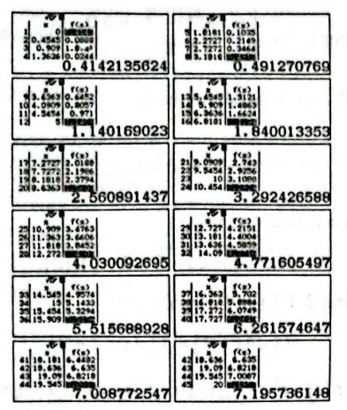
\includegraphics[width=0.65\textwidth]{anh3.png}
\end{center}

\vspace{0.3cm}
\noindent Dựa vào bảng tính, $f(x)$ không đổi dấu với 45 giá trị tính trên bảng, tức đồ thị hàm số $f(x)$ không cắt trục hoành (trên 45 giá trị đầu), mà gần như xấp xỉ bằng 0 từ thứ tự 0 đến 12 của $x$ và tăng dần đều đến thứ tự 45, qua đó ta có nhận định tại giá trị $x_0$ thuộc $[0;1]$ đồ thị hàm số $f(x)$ có xu hướng tiếp xúc với trục hoành tại điểm $x_0$ (khả năng có nghiệm bội), dùng chức năng \textbf{SOLVE (SHIFT CALC)} để tìm nghiệm $x_0$ của PT(4.3) trên đoạn $[0;1]$, với giá trị "khởi tạo" chẳng hạn tại $x=0.5$ (vì giá trị này gần với nghiệm $x_0$), tìm được $x_0=1$, tiếp tục tìm các nghiệm còn lại bằng cách chia $f(x)$ cho $(x-1)$ và ấn \textbf{SHIFT CALC} chờ máy giải thì kết quả màn hình hiển thị "không giải được".

\vspace{0.4cm}
\begin{center}
    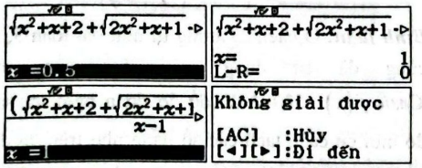
\includegraphics[width=0.7\textwidth]{anh4.png}
\end{center}
\noindent PT(4.3) chỉ có nghiệm $x_0 = 1$ và có thể là nghiệm bội hai, ta tách nhân tử cho từng căn thức theo công thức sau:
\[
\begin{cases} f(x_0) = ax_0 + b \\ f'(x_0) = a \end{cases}, \, x_0 = 1; \, a, b \in \mathbb{R}, \text{ a, b là ẩn số cần tìm.}
\]

\noindent Với $f(x)$ lần lượt là $\sqrt{k^2 + k + 2}$ và $\sqrt{2k^2 + k + 1}$, thực hiện cách tìm a,b hai lần khi đó ta có cách tách các số hạng như ở cách 2.

\vspace{0.2cm}
\noindent \textbf{Nhận xét:}

\noindent Phương trình thứ nhất của hệ chứa các căn thức đồng bậc:
\[
\sqrt{x^2 + xy + 2y^2}, \sqrt{y^2 + xy + 2x^2},
\]
nên ta đặt $x = ky$.

\noindent Sau phép đặt, bài toán được quy về phương trình một ẩn $k$, từ đó suy ra quan hệ
\[
x = y.
\]

\noindent Đặc biệt, bài toán cho thấy cùng một phương trình có thể được xử lí bằng nhiều hướng khác nhau như:

\vspace{0.2cm}
\noindent $\bullet$ bình phương hai vế;

\vspace{0.1cm}
\noindent $\bullet$ dùng liên hợp;

\vspace{0.1cm}
\noindent $\bullet$ sử dụng tính đơn điệu của hàm số.

\vspace{0.2cm}
\noindent Điều này thể hiện tính linh hoạt của phương pháp đặt ẩn phụ tỉ lệ khi kết hợp với các công cụ đại số khác.

\vspace{0.4cm}
\noindent \textbf{Bài toán 5.} \textit{Giải hệ phương trình}
\[
(5^*): \begin{cases}
\dfrac{1}{x} + \dfrac{1}{y} + \dfrac{1}{z} = \dfrac{1}{xyz} \quad (5.1) \\[10pt]
x + y + z = xyz + \dfrac{8}{27}(x + y + z)^3 \quad (5.2)
\end{cases}
\]
\begin{itemize}
    \item[\textbf{1.}] \textbf{Hướng giải (Vì sao đưa ra bài toán này):} 
    Khi số lượng biến tăng lên thành 3 ẩn với tính đối xứng cao, phương pháp ẩn phụ tỉ lệ thông thường cần được nâng cấp. Bài toán đặt ra nhằm mở rộng mô hình: đặt đồng thời $y = kx$ và $z = lx$ ($k, l \neq 0$). Quá trình thay thế giúp chuyển hệ 3 ẩn ban đầu thành hệ 2 ẩn $k, l$, sau đó tiếp tục sử dụng ẩn phụ Tổng - Tích ($S = k+l, P = kl$) để giải quyết triệt để.

    \item[\textbf{2.}] \textbf{Cái hay của bài toán:} 
    Đây là mô hình mẫu mực cho \textbf{chuỗi ẩn phụ liên tiếp nhiều tầng} (tỉ lệ $\rightarrow$ tổng - tích). Bài toán minh họa của các hệ phương trình nhiều biến phức tạp mà không bị rối.
\end{itemize}
\vspace{0.2cm}
\noindent \textbf{Lời giải.} ĐK: $\begin{cases} x \neq 0 \\ y \neq 0 \\ z \neq 0 \end{cases}$. Giả sử có $\begin{cases} y = kx \\ z = lx \end{cases}$, từ ĐK ta có $k, l \neq 0$, với $k, l$ là ẩn số phụ, dễ thấy các biến số thỏa mãn MỆNH ĐỀ 1.3.1 -- (2.i) nên ta có thể đặt:

\vspace{0.2cm}
\noindent $(5^*1): \begin{cases} y = kx \\ z = lx \end{cases}$, $k, l \in \mathbb{R} \setminus \{0\}$ và thay vào PT(5.1), PT(5.2), biến đổi và thu gọn, ta được:
\[
\begin{cases}
x^2 = \dfrac{1}{kl + k + l}, \, kl + k + l > 0 \\[10pt]
x^2 \left[ kl + \dfrac{8}{27}(1 + k + l)^3 \right] = 1 + k + l
\end{cases}
\]
\[
\Leftrightarrow (5^*2): \begin{cases}
kl + k + l > 0 \\
27kl + 8(1 + k + l)^3 = 27(1 + k + l)(kl + k + l)
\end{cases}
\]

\vspace{0.2cm}
\noindent Tiếp tục đặt $\begin{cases} S = k + l \\ P = kl \end{cases}$ ta có hệ ($5^*2$) trở thành
\[
\begin{cases}
S + P > 0 \\
27P + 8(1 + S)^3 = 27(1 + S)(P + S)
\end{cases} \quad (5.3)
\]

\noindent Ta có điều kiện để PT(5.3) có nghiệm là
\[
(5^*3): \begin{cases} S^2 - 4P \geq 0 \quad (5.4) \\ S + P > 0 \quad\ \ (5.5) \end{cases}
\]

\noindent Thu gọn PT(5.3) ta được PT tương đương:
\[
27SP = 8S^3 - 3S^2 - 3S + 8 \quad (5.6).
\]

\noindent Ta xét các khả năng của PT(5.6) như sau:

\vspace{0.2cm}
\noindent \textbf{TH1.} Xét $S = 0$, rõ ràng PT(5.6) không thỏa mãn.

\vspace{0.2cm}
\noindent \textbf{TH2.} Xét $S \neq 0$, ta chia hai vế PT(5.6) cho $27S$, ta được:
\[
P = \dfrac{8S^3 - 3S^2 - 3S + 8}{27S}
\]
\[
= \dfrac{(S + 1) \left[ 8\left(S - \dfrac{11}{16}\right)^2 + \dfrac{135}{32} \right]}{27S} \quad (5.7).
\]

\noindent Từ PT(5.7) ta xét:

\vspace{0.2cm}
\noindent $\bullet$ Nếu $S > 0$ thì $P > 0$ khi đó $S + P > 0$ thỏa mãn ĐK(5.5), ta thay P bởi vế phải PT(5.7) vào ĐK(5.4) kết hợp $S > 0$ ta có:
\[
\begin{cases} S > 0 \\ S^2 - 4P \geq 0 \end{cases} \Leftrightarrow \begin{cases} S > 0 \\ S^2 - 4 \cdot \dfrac{8S^3 - 3S^2 - 3S + 8}{27S} \geq 0 \end{cases}
\]
\[
\Leftrightarrow \begin{cases} S > 0 \\ \dfrac{-(S - 2)^2(25S + 8)}{27S} \geq 0 \end{cases} \Leftrightarrow S = 2.
\]
\noindent Thay $S = 2$ vào vế phải PT(5.7) tính được $P = 1$, khi đó $\begin{cases} S = k + l = 2 \\ P = kl = 1 \end{cases} \Leftrightarrow k = l = 1$, kết hợp với ($5^*1$) ta có $\begin{cases} y = x \\ z = x \end{cases}$, thay vào (5.1) ta được:

\vspace{0.2cm}
\noindent $\dfrac{3}{x} = \dfrac{1}{x^3} \Leftrightarrow \begin{cases} x \neq 0 \\ x^2 = \dfrac{1}{3} \end{cases} \Leftrightarrow x = \pm \dfrac{1}{\sqrt{3}} \implies y = z = \pm \dfrac{1}{\sqrt{3}}$

\vspace{0.3cm}
\noindent $\bullet$ Nếu $S = -1$ thì $P = 0$ khi đó:
\[
\begin{cases} S = k + l = -1 \\ P = kl = 0 \end{cases} \Leftrightarrow \begin{cases} k = -1 \\ l = 0 \end{cases} \text{ hoặc } \begin{cases} k = 0 \\ l = -1 \end{cases} \text{ (không thỏa mãn ĐK nên loại).}
\]

\noindent $\bullet$ Nếu $-1 < S < 0$ thì $P < 0$, khi đó rõ ràng $S + P < 0$ không thỏa mãn ĐK(5.5) nên loại.

\vspace{0.2cm}
\noindent $\bullet$ Nếu $S < -1$ thì $P > 0$, ta có 3 khả năng:

\vspace{0.1cm}
\noindent $\bullet$ Nếu hệ ($5^*3$) có (5.4) thỏa mãn, (5.5) không thỏa mãn thì ta loại.

\vspace{0.1cm}
\noindent $\bullet$ Nếu hệ ($5^*3$) có (5.5) thỏa mãn, (5.4) không thỏa mãn thì ta loại.

\vspace{0.1cm}
\noindent $\bullet$ Nếu hệ ($5^*3$) thỏa mãn cả 2 ĐK (5.4) và (5.5), khi đó ta có lập luận:
\[
S < -1 \Leftrightarrow 0 < S + P < -1 + P \implies P > 1 \quad (5.8).
\]

\noindent Từ (5.4) ta có: $S^2 \geq 4P$ và $P > 0$, lấy căn bậc 2 hai vế của $S^2 \geq 4P$ được:
\[

|S| \geq 2\sqrt{P} \Leftrightarrow \left[ 
\begin{aligned}
&S \geq 2\sqrt{P} \quad (5.9) \\
&S \leq -2\sqrt{P} \quad (5.10)
\end{aligned} 
\right.
\]

\noindent $-$ Xét trường hợp có (5.9) kết hợp với $S < -1$ ta có: $2\sqrt{P} \leq S < -1 \Leftrightarrow \sqrt{P} < \dfrac{1}{2}$, mâu thuẫn với (5.8) nên loại.

\vspace{0.2cm}
\noindent $-$ Xét trường hợp có (5.10) kết hợp với $S < -1$ ta có: $\left[ \begin{aligned} &S \leq -1 \\ &S \leq -2\sqrt{P} \end{aligned} \right. \Leftrightarrow -1 < -2\sqrt{P} \Leftrightarrow \sqrt{P} < \dfrac{1}{2}$, mâu thuẫn với (5.8) nên loại.

\vspace{0.3cm}
\noindent \textbf{Kết luận:} $HPT(5^*)$ có hai nghiệm là
\[
(x;y;z) \in \left\{ \left( \dfrac{1}{\sqrt{3}}; \dfrac{1}{\sqrt{3}}; \dfrac{1}{\sqrt{3}} \right); \left( \dfrac{-1}{\sqrt{3}}; \dfrac{-1}{\sqrt{3}}; \dfrac{-1}{\sqrt{3}} \right) \right\}
\]

\noindent \textbf{Nhận xét:}

\noindent Đây là ví dụ tiêu biểu cho trường hợp đặt nhiều ẩn theo cùng một biến:
\[
y = kx, z = lx.
\]
\noindent Sau phép đặt, hệ phương trình được đưa về các biểu thức đối xứng theo $k, l$, từ đó tiếp tục sử dụng phép đặt:
\[
S = k + l, P = kl
\]
\noindent để khai thác cấu trúc đối xứng của bài toán.

\vspace{0.2cm}
\noindent Bài toán cho thấy phương pháp đặt ẩn phụ tỉ lệ có thể kết hợp hiệu quả với phương pháp sử dụng tổng và tích nghiệm nhằm giảm đáng kể độ phức tạp của hệ phương trình.
\newpage
\noindent \textbf{CHƯƠNG 3. ỨNG DỤNG TRONG BÀI TOÁN TÌM GIÁ TRỊ LỚN NHẤT, GIÁ TRỊ NHỎ NHẤT}

\vspace{0.3cm}
\noindent 
Trong mục này, ta giải bài toán tìm GTLN, GTNN của biểu thức hai biến số, ba biến số, với các điều kiện ràng buộc cho trước, theo cách đặt ẩn phụ, ta có phương pháp sau:

\vspace{0.2cm}
\noindent \textbf{Phương pháp chung:} Dựa vào các điều kiện của Mệnh đề 1.2.1 hoặc Mệnh đề 1.3.1 và biểu thức cần tìm GTLN, GTNN, kết hợp điều kiện ràng buộc, ta đặt ẩn phụ sao cho phù hợp, lưu ý rằng cần xác định miền xác định của ẩn số phụ thật chính xác, lúc đó quy bài toán hai biến, ba biến về khảo sát bài toán tìm GTLN, GTNN của hàm một biến số trên một đoạn, một khoảng quen thuộc trong sách giáo khoa Toán 12 hoặc có thể tìm GTLN, GTNN bằng các bất đẳng thức cổ điển như bất đẳng thức Cauchy, Bunyakovsky, ... với lưu ý rằng cần đoán được dấu "=" trong từng bài toán, khi đó ta mới vận dụng được.

\vspace{0.4cm}
\noindent \textbf{Bài toán 6.} \textit{Cho các số thực dương $x, y$. Xác định giá trị lớn nhất của biểu thức}
\[
A = \dfrac{xy}{\left(x + \sqrt{x^2 + y^2}\right)^2}.
\]

\begin{itemize}
    \item[\textbf{1.}] \textbf{Hướng giải (Vì sao đưa ra bài toán này):} 
    Nhận diện biểu thức $A$ có tính thuần nhất (tử và mẫu cùng bậc), bài toán được đưa ra nhằm rèn luyện kỹ năng khử biến bằng phép đặt ẩn phụ tỉ lệ $x = ky$ ($k > 0$). Thao tác này giúp đưa bài toán tìm cực trị của hàm hai biến $x, y$ về khảo sát hàm số một biến $f(k)$ trên khoảng $(0, +\infty)$.

    \item[\textbf{2.}] \textbf{Cái hay của bài toán:} 
    Điểm sáng là kỹ thuật \textbf{biến đổi mẫu số bằng lượng liên hợp}: $\frac{1}{k+\sqrt{k^2+1}} = \sqrt{k^2+1}-k$. Phép biến đổi này đã biến một mẫu số chứa căn phức tạp thành dạng đa thức/căn thức gọn gàng, giúp việc tính đạo hàm và lập bảng biến thiên.
\end{itemize}
\vspace{0.2cm}
\noindent \textbf{Lời giải.} Giả sử có $x = ky$, và với $x, y$ là các số thực dương thì $k > 0$, với $k$ là ẩn số phụ, khi đó các biến số thỏa mãn MỆNH ĐỀ 1.2.1 -- (1.i) nên ta có thể đặt $x = ky$, $k > 0$, thay vào biểu thức A để được:
\[
A = \dfrac{(ky)y}{\left(ky + \sqrt{(ky)^2 + y^2}\right)^2} \overset{y > 0}{\Leftrightarrow} \dfrac{k}{\left(k + \sqrt{k^2 + 1}\right)^2} := f(k) \quad (6.1).
\]

\vspace{0.2cm}
\noindent Ta có: $\begin{cases} k + \sqrt{k^2 + 1} > 0, \forall k > 0 \\ (k + \sqrt{k^2 + 1})(k - \sqrt{k^2 + 1}) = k^2 - (k^2 + 1) = -1 \end{cases}$
\[
\implies \dfrac{1}{k + \sqrt{k^2 + 1}} = \sqrt{k^2 + 1} - k \quad (6.2).
\]

\noindent Từ (6.2), ta biến đổi hàm số $f(k)$ trở thành:
\[
f(k) = k \left(\sqrt{k^2 + 1} - k\right)^2 = 2k^3 + k - 2k^2\sqrt{k^2 + 1}
\]

\noindent Khi đó, lấy đạo hàm cấp 1 và đạo hàm cấp 2 hàm số $f(k)$ và thu gọn, nhận được:
\[
f'(k) = 6k^2 + 1 - \dfrac{6k^3 + 4k}{\sqrt{k^2 + 1}}.
\]
\[
f''(k) = 12k - \dfrac{12k^4 + 18k^2 + 4}{\left(\sqrt{k^2+1}\right)^3}.
\]

\noindent Ta có: $f'(k) = 0 \Leftrightarrow \begin{cases} k > 0 \\ (6k^2 + 1)^2(k^2 + 1) = (6k^3 + 4k)^2 \end{cases}$
\[
\Leftrightarrow \begin{cases} k > 0 \\ 3k^2 = 1 \end{cases} \Leftrightarrow k_0 = \dfrac{1}{\sqrt{3}}.
\]

\noindent $f\left(\dfrac{1}{\sqrt{3}}\right) = \dfrac{\sqrt{3}}{9}$, $f(0) = 0$; $\lim\limits_{k \to +\infty} f(k) = \lim\limits_{k \to +\infty} \dfrac{k}{\left(k + \sqrt{k^2+1}\right)^2}$
\[
= \lim\limits_{k \to +\infty} \dfrac{\dfrac{1}{k}}{\left(1 + \sqrt{1 + \dfrac{1}{k^2}}\right)^2} = 0.
\]

\vspace{0.2cm}
\noindent Lại có $f''\left(\dfrac{1}{\sqrt{3}}\right) = -\dfrac{\sqrt{3}}{4} < 0$, do đó $k_0 = \dfrac{1}{\sqrt{3}}$ là điểm cực đại của hàm số $f(k)$ trên khoảng $(0; +\infty)$.

\vspace{0.4cm}
% --- BẢNG BIẾN THIÊN ---
\begin{center}
\renewcommand{\arraystretch}{1.5}
\begin{tabular}{|c|lcr|}
\hline
$k$ & $0$ & $\frac{1}{\sqrt{3}}$ & $+\infty$ \\ \hline
$f'(k)$ & \quad $+$ & $0$ & $-$ \quad \\ \hline
 & & $\dfrac{\sqrt{3}}{9}$ & \\
$f(k)$ & & $\nearrow \quad \quad \quad \searrow$ & \\
 & $0$ & & $0$ \\ \hline
\end{tabular}
\end{center}
\vspace{0.4cm}

\noindent Từ bảng biến thiên và (6.1) ta thấy:
\[
\max_{x>0, y>0} A = \max_{k \in (0; +\infty)} f(k) = f\left(\dfrac{1}{\sqrt{3}}\right) = \dfrac{\sqrt{3}}{9}
\]
\noindent với $k = \dfrac{1}{\sqrt{3}} \overset{x=ky}{\implies} x = \dfrac{1}{\sqrt{3}}y$.

\vspace{0.2cm}
\noindent \textbf{Kết luận:} $\max A = \dfrac{\sqrt{3}}{9}$ tại $(x; y) = \left(\dfrac{1}{\sqrt{3}}y; y\right)$; $y > 0$.

\vspace{0.3cm}
\noindent \textbf{Nhận xét:}

\noindent Nếu hàm số $y = f(x)$ có đạo hàm liên tục đến cấp hai trong một lân cận của $x_0$, đồng thời $f'(x_0) = 0, f''(x_0) \neq 0$, thì:

\vspace{0.2cm}
\noindent $\bullet$ Nếu $f''(x_0) < 0$, thì hàm số đạt \textbf{cực đại} tại $x_0$.

\vspace{0.1cm}
\noindent $\bullet$ Nếu $f''(x_0) > 0$, thì hàm số đạt \textbf{cực tiểu} tại $x_0$.

\vspace{0.2cm}
\noindent Định lí này giúp ta khẳng định được $x_0$ là điểm cực đại hay điểm cực tiểu khi không xét dấu được $f'(x)$ hoặc giúp cho lời giải bài toán được chặt chẽ hơn. Nếu
\noindent giả thiết bài toán 6 được thay bởi x, y là hai số thực không âm và không đồng thời bằng 0, với lưu ý cần xét khả năng MỆNH ĐỀ 1.2.1 -- (1.ii) trước khi đặt ẩn phụ thì khi đó ta còn tìm được GTNN của biểu thức A bằng 0 đạt được tại
\[
\begin{cases} x_0 = 0 \\ y_0 > 0 \end{cases} \text{ hoặc } \begin{cases} y_0 = 0 \\ x_0 > 0 \end{cases}.
\]
Hãy nghiên cứu thật kĩ nội dung trên và phân tích vào từng bài toán, các bài này thầy tôi yêu cầu không phải chỉ đơn giản đưa ra lời giải mà phải nêu hướng giải vì sao lại đưa ra bài đó, cái hay của mỗi bài
\vspace{0.4cm}
\noindent \textbf{Bài toán 7.} \textit{Cho các số thực dương x, y thỏa mãn}
\[
(7^*): \begin{cases}
x < \sqrt{2}y \quad (7.1) \\
x\sqrt{y^2 - \dfrac{x^2}{2}} = 2\sqrt{y^2 - \dfrac{x^2}{4}} + x \quad (7.2)
\end{cases}
\]

\begin{itemize}
    \item[\textbf{1.}] \textbf{Hướng giải (Vì sao đưa ra bài toán này):} 
    Dựa trên giả thiết có chứa miền giá trị lệch ($x < \sqrt{2}y$), bài toán yêu cầu học sinh sử dụng ẩn phụ tỉ lệ $x = ky$ để đưa giả thiết về mối quan hệ giữa $k$ và $y$. Tiếp đó, kết hợp đặt ẩn phụ trung gian cho biểu thức căn thức để quy đổi biểu thức $B$ về một hàm số tối ưu theo ẩn mới.

    \item[\textbf{2.}] \textbf{Cái hay của bài toán:} 
    Minh chứng tiêu biểu cho kỹ thuật \textbf{ẩn phụ kép nhiều tầng}. Bài toán rèn luyện sự tinh tế trong việc định hình điểm rơi, tạo ra dạng biểu thức gọn gàng để áp dụng trực tiếp bất đẳng thức Cauchy.
\end{itemize}
\vspace{0.2cm}
\noindent \textit{Tìm GTNN của biểu thức $B = x^2\sqrt{y^2 - \dfrac{x^2}{2}}$.}

\vspace{0.3cm}
\noindent \textbf{Lời giải.} Giả sử có $x = ky$, và với $x, y$ là các số thực dương thì $k > 0$, với $k$ là ẩn số phụ, khi đó các biến số thỏa mãn MỆNH ĐỀ 1.2.1 -- (1.i) nên ta có thể đặt $x = ky$, $k > 0$ thay vào giả thiết ($7^*$) và biểu thức B, biến đổi, nhận được:
\[
\begin{cases}
x < \sqrt{2}(kx), \, x > 0 \\
x\sqrt{(kx)^2 - \dfrac{x^2}{2}} = 2\sqrt{(kx)^2 - \dfrac{x^2}{4}} + x
\end{cases}
\implies \begin{cases}
k > \dfrac{1}{\sqrt{2}} \hfill (7.3) \\[10pt]
x = \dfrac{2\sqrt{k^2 - \dfrac{1}{4}} + 1}{\sqrt{k^2 - \dfrac{1}{2}}} \hfill (7.4)
\end{cases}
\]

\vspace{0.2cm}
\noindent Biến đổi biểu thức B kết hợp cùng (7.3) và (7.4), ta có:
\[
B = x^2\sqrt{(kx)^2 - \dfrac{x^2}{2}} \overset{x > 0}{\Leftrightarrow} x^3\sqrt{k^2 - \dfrac{1}{2}}
\]
\[
\overset{(7.4)}{\Leftrightarrow} \left( \dfrac{2\sqrt{k^2 - \dfrac{1}{4}} + 1}{\sqrt{k^2 - \dfrac{1}{2}}} \right)^3 \times \sqrt{k^2 - \dfrac{1}{2}} \overset{(7.3)}{\Leftrightarrow} \dfrac{\left(2\sqrt{k^2 - \dfrac{1}{4}} + 1\right)^3}{k^2 - \dfrac{1}{2}}.
\]

\vspace{0.2cm}
\noindent Lại đặt $t = \sqrt{k^2 - \dfrac{1}{4}}$ với $k > \dfrac{1}{\sqrt{2}}$ thì $t > \dfrac{1}{2}$. Vì vậy, biểu thức B tiếp tục được biến đổi trở thành:
\[
B = \dfrac{4(2t + 1)^3}{4t^2 - 1} = \dfrac{4(2t + 1)^2}{2t - 1}
\]
\[
= 4 \left[ (2t - 1) + \dfrac{4}{2t - 1} + 4 \right].
\]

\vspace{0.2cm}
\noindent Áp dụng BĐT Cauchy ta có:
\[
B \geq 4 \times \left[ 2\sqrt{(2t - 1) \times \dfrac{4}{2t - 1}} + 4 \right]
\]
\[
= 4 \times (2.2 + 4) = 32.
\]

\noindent Đẳng thức xảy ra khi $\begin{cases} t > \dfrac{1}{2} \\[10pt] 2t - 1 = \dfrac{4}{2t - 1} \end{cases} \Leftrightarrow t = \dfrac{3}{2}$,

\vspace{0.2cm}
\noindent kết hợp với $\begin{cases} t = \sqrt{k^2 - \dfrac{1}{4}} \\[10pt] k > \dfrac{1}{\sqrt{2}} \end{cases}$ tìm được $k = \dfrac{\sqrt{10}}{2}$,

\vspace{0.2cm}
\noindent tiếp tục sử dụng (7.4) và $y = kx$, ta tìm được:
\[
x = 2\sqrt{2}, \, y = 2\sqrt{5}.
\]

\noindent \textbf{Kết luận:} $\min B = 32$ khi $(x; y) = (2\sqrt{2}; 2\sqrt{5})$.

\vspace{0.2cm}
\noindent \textbf{Nhận xét:} Không sử dụng BĐT Cauchy, ta vẫn có thể lập BBT như bài toán 6 để giải, trong đó ta cần lưu ý với $t > \dfrac{1}{2}$ thì $B'(t) = \dfrac{8(4t^2 - 4t - 3)}{(2t - 1)^2}$; $B'(t) = 0 \Leftrightarrow t = \dfrac{3}{2}$, khi đó $B'(t)$ đổi dấu từ "$-$" sang "$+$" khi qua giá trị $t = \dfrac{3}{2}$, kết hợp $\lim\limits_{t \to \left(\dfrac{1}{2}\right)^+} \dfrac{4(2t + 1)^2}{2t - 1} = +\infty$ và $\lim\limits_{t \to +\infty} \dfrac{4(2t + 1)^2}{2t - 1} = +\infty$ bài toán mới được khảo sát đúng.

\vspace{0.4cm}
\noindent \textbf{Bài toán 8.} \textit{Chứng minh rằng với mọi số thực dương x, y, z thỏa mãn $x(x + y + z) = 3yz$ (8.1) ta có: $C = (x + y)^3 + (x + z)^3 + 3(x + y)(y + z)(z + x) - 5(y + z)^3 \leq 0$.}

\begin{itemize}
    \item[\textbf{1.}] \textbf{Hướng giải (Vì sao đưa ra bài toán này):} 
    Nhận thấy giả thiết và biểu thức $C$ đều mang tính thuần nhất, đặt ẩn phụ tỉ lệ 2 ẩn theo 1 ẩn ($y = kx, z = lx$). Từ giả thiết, ta rút ra mối liên hệ giữa $k$ và $l$, sau đó thay toàn bộ vào $C$ để chuyển bất đẳng thức 3 biến thành việc khảo sát hàm số một biến $f(k) \le 0$.

    \item[\textbf{2.}] \textbf{Cái hay của bài toán:} 
    Giải quyết triệt để sự cồng kềnh của bất đẳng thức 3 biến bằng công cụ đạo hàm. Lời giải tránh được hoàn toàn nguy cơ ngược dấu hay sai điểm rơi thường gặp khi dùng các bất đẳng thức cổ điển.
\end{itemize}
\vspace{0.3cm}
\noindent \textbf{Lời giải.} Giả sử có $\begin{cases} y = kx \\ z = lx \end{cases}$, và với $x, y, z$ là các số thực dương thì $k, l > 0$, với $k, l$ là các ẩn số phụ, khi đó các biến số thỏa mãn MỆNH ĐỀ 1.3.1 -- (2.i) nên ta đặt: ($8^*1$) $\begin{cases} y = kx \\ z = lx \end{cases}$; $k, l > 0$, thay vào (8.1), ta được:
\[
x(x + kx + lx) = 3(kx)(lx) \overset{x > 0}{\Leftrightarrow} 1 + k + l = 3kl \quad (8.2).
\]

\noindent Áp dụng BĐT Cauchy, kết hợp cùng (8.2) ta có:
\[
3kl = 1 + k + l \geq 2\sqrt{kl} + 1
\]
\[
\Leftrightarrow 3(\sqrt{kl})^2 - 2\sqrt{kl} - 1 \geq 0
\]
\[
\Leftrightarrow \left[ 
\begin{aligned}
&\sqrt{kl} \geq 1 \Leftrightarrow kl \geq 1 \quad (8.3) \\
&\sqrt{kl} \leq -\dfrac{1}{3} \text{ (không tồn tại } kl)
\end{aligned} 
\right.
\]

\noindent Tiếp tục thay ($8^*1$) vào BĐT $C \leq 0$, ta có:
\[
C = (x + kx)^3 + (x + lx)^3 + 3(x + kx)(kx + lx)(lx + x) - 5(kx + lx)^3 \leq 0
\]
\[
\Leftrightarrow C = x^3(1 + k)^3 + x^3(1 + l)^3 + 3x^3(1 + k)(k + l)(l + 1) - 5x^3(k + l)^3 \leq 0 \quad (8.4).
\]

\noindent Vì x, k, l là các số dương, nên ta chia hai vế BĐT (8.4) cho $(k + l)^3 > 0$ và đơn giản cho $x^3 > 0$, tiếp tục sử dụng hằng đẳng thức
\[
a^3 + b^3 = (a + b)^3 - 3ab(a + b) \text{ và (8.2) ta có:}
\]
\[
C(k, l) = \left(\dfrac{1 + k}{k + l}\right)^3 + \left(\dfrac{1 + l}{k + l}\right)^3 + 3\left(\dfrac{1 + k}{k + l}\right)\left(\dfrac{1 + l}{k + l}\right) - 5 \leq 0
\]
\[
\Leftrightarrow C(k, l) = \left(\dfrac{2 + k + l}{k + l}\right)^3 - 6 \times \dfrac{1 + k + l + kl}{(k + l)^2} - 5 \leq 0
\]
\[
\overset{(8.2)}{\implies} C(k, l) = \left(\dfrac{1 + 3kl}{3kl - 1}\right)^3 - \dfrac{24kl}{(3kl - 1)^2} - 5 \leq 0 \quad (8.5).
\]

\noindent Ta đặt $t = kl$, khi đó từ BĐT (8.3) và BĐT (8.5), ta có:
\[
f(t) := \left(\dfrac{1 + 3t}{3t - 1}\right)^3 - \dfrac{24t}{(3t - 1)^2} - 5; \, t \geq 1.
\]

\noindent Ta có: $f'(t) = 3 \cdot \dfrac{-6}{(3t - 1)^2} \cdot \left(\dfrac{3t + 1}{3t - 1}\right)^2 - 24 \cdot \dfrac{(3t - 1)^2 - (3t) \cdot 2 \cdot 3 \cdot (3t - 1)}{(3t - 1)^4}$
\[
= \dfrac{-162t^2 + 36t + 6}{(3t - 1)^4} = \dfrac{-6(9t + 1)}{(3t - 1)^3} < 0, \, \forall t \in [1; +\infty).
\]

\noindent Suy ra $f(t)$ là hàm số nghịch biến trên $[1; +\infty)$.

\noindent Do đó, với $t \geq 1$ thì
\[
f(t) \leq f(1) = 0 \text{ hay } \max_{t \in [1; +\infty)} f(t) = f(1) = 0 \quad (8.6).
\]

\noindent Từ (8.6) rõ ràng ta đã chứng minh được BĐT (8.5) tức BĐT $C \leq 0$ đã được chứng minh.

\noindent Dấu "=" xảy ra ở BĐT $C \leq 0$ khi và chỉ khi:
\[
\begin{cases} t = kl = 1 \\ 1 + k + l = 3kl \end{cases} \Leftrightarrow \begin{cases} k + l = 2 \\ kl = 1 \end{cases} \Leftrightarrow k = l = 1
\]
\[
\overset{(8^*1)}{\implies} x = y = z > 0.
\]
\vspace{0.4cm}
\noindent \textbf{Bài toán 9.} \textit{Cho các số thực dương $x, y, z$ thỏa mãn điều kiện}
\[
x^2 + y^2 - 2z^2 + 2xy + yz + zx \leq 0 \quad (9.1).
\]
\noindent \textit{Tìm giá trị nhỏ nhất của biểu thức}
\[
D = \dfrac{x^4 + y^4}{z^4} + \dfrac{y^4 + z^4}{x^4} + \dfrac{z^4 + x^4}{y^4}.
\]

\begin{itemize}
    \item[\textbf{1.}] \textbf{Hướng giải (Vì sao đưa ra bài toán này):} 
    Bài toán được tạo ra nhằm rèn luyện kỹ năng phân tích nhân tử để rút gọn giả thiết bất phương trình thành dạng tích $(x+y+2z)(x+y-z) \le 0$, suy ra $x+y \le z$. Kết hợp tính thuần nhất bậc 0 của biểu thức $D$, ta đặt ẩn phụ tỉ lệ $x = kz, y = lz$ với $k+l \le 1$ để đưa biểu thức về dạng hàm số theo hai biến $k, l$.

    \item[\textbf{2.}] \textbf{Cái hay của bài toán:} 
    Sự kết hợp giữa \textbf{phân tích giả thiết $\rightarrow$ chuẩn hóa ẩn phụ tỉ lệ $\rightarrow$ đánh giá Cauchy điểm rơi}. Miền giá trị được thu hẹp gọn gàng ($k+l \le 1$), giúp việc tìm giá trị nhỏ nhất.
\end{itemize}
\vspace{0.2cm}
\noindent \textbf{Lời giải.} Ta có với $x, y, z > 0$ thì:
\[
(9.1) \Leftrightarrow (x + y)^2 - z(x + y) + 2z(y + x) - 2z^2 \leq 0
\]
\[
\Leftrightarrow (x + y)(x + y - z) + 2z(y + x - z) \leq 0
\]
\[
\Leftrightarrow (x + y + 2z)(x + y - z) \leq 0 \Leftrightarrow x + y \leq z \quad (9.2).
\]

\vspace{0.2cm}
\noindent Giả sử có $\begin{cases} x = kz \\ y = lz \end{cases}$, và với $x, y, z$ là các số thực dương thì $k, l > 0$, với $k, l$ là các ẩn số phụ, khi đó các biến số thỏa mãn MỆNH ĐỀ 1.3.1 -- (2.i) nên ta có thể đặt:
\[
(9^*): \begin{cases} 0 < x = kz \\ 0 < y = lz \end{cases}; \, k, l > 0.
\]

\noindent Thay hệ ($9^*$) vào BĐT (9.2) ta được:
\[
0 < kz + lz \leq z \overset{z > 0}{\Leftrightarrow} 0 < k + l \leq 1 \quad (9.3).
\]

\noindent Thay hệ ($9^*$) vào biểu thức D và rút gọn, ta được:
\[
D(k, l) = \left( \underbrace{k^4 + l^4}_{D_1(k, l)} \right) + \left( \underbrace{\dfrac{1}{k^4} + \dfrac{1}{l^4}}_{D_2(k, l)} \right) + \left( \underbrace{\dfrac{l^4}{k^4} + \dfrac{k^4}{l^4}}_{D_3(k, l)} \right).
\]

\vspace{0.2cm}
\noindent Theo BĐT Cauchy ta có:
\[
D_3(k, l) = \dfrac{l^4}{k^4} + \dfrac{k^4}{l^4} \geq 2\sqrt{\dfrac{l^4}{k^4} \times \dfrac{k^4}{l^4}} = 2 \quad (9.4);
\]
\[
D_2(k, l) = \dfrac{1}{k^4} + \dfrac{1}{l^4} \geq \dfrac{2}{k^2l^2} \geq \dfrac{2}{\left[ \left(\dfrac{k + l}{2}\right)^2 \right]^2} = \dfrac{32}{(k + l)^4} \quad (9.5);
\]
\[
D_1(k, l) = \left( k^4 + \dfrac{1}{16} + \dfrac{1}{16} + \dfrac{1}{16} \right) + \left( l^4 + \dfrac{1}{16} + \dfrac{1}{16} + \dfrac{1}{16} \right) - \dfrac{3}{8} \quad (9.6).
\]

\[
\geq 4\sqrt[4]{\dfrac{k^4}{16^3}} + 4\sqrt[4]{\dfrac{l^4}{16^3}} - \dfrac{3}{8} = \dfrac{k + l}{2} - \dfrac{3}{8} \quad (9.6).
\]

\noindent Cộng theo vế ba BĐT (9.4), (9.5), (9.6) thu được:
\[
D(k,l) = D_1(k,l) + D_2(k,l) + D_3(k,l)
\]
\[
\geq \left(\dfrac{k + l}{2} - \dfrac{3}{8}\right) + \dfrac{32}{(k + l)^4} + 2
\]
\[
\Leftrightarrow D(k,l) \geq \dfrac{32}{(k + l)^4} + \dfrac{k + l}{2} - \dfrac{13}{8} \quad (9.7).
\]

\noindent Đặt $t = k + l$, từ vế phải BĐT (9.7) và BĐT (9.3) ta có:
\[
f(t) := \dfrac{32}{t^4} + \dfrac{t}{2} + \dfrac{13}{8}; \, 0 < t \leq 1. \text{ Khi đó:}
\]
\[
f'(t) = \dfrac{1}{2} - \dfrac{128}{t^5} \leq -\dfrac{255}{2} < 0, \, \forall t \in (0; 1].
\]

\noindent Suy ra $f(t)$ là hàm số nghịch biến trên $(0; 1]$, do đó:
\[
\min_{t \in (0; 1]} f(t) = f(1) = \dfrac{273}{8} \quad (9.8).
\]

\noindent Từ (9.7) và (9.8), ta suy ra được $D(k,l) \geq f(t) \geq \dfrac{273}{8}$. Đẳng thức xảy ra khi và chỉ khi đẳng thức ở (9.4), (9.5), (9.6), (9.7) và (9.8) cùng đồng thời xảy ra:
\[
\begin{cases}
k; l > 0 \\
k^4 = l^4 = \dfrac{1}{16} \\[8pt]
\dfrac{l^4}{k^4} + \dfrac{k^4}{l^4} = 4; \dfrac{1}{k^4} = \dfrac{1}{l^4}; k = l \\[8pt]
k + l = 1
\end{cases}
\Leftrightarrow k = l = \dfrac{1}{2} \implies x = y = \dfrac{z}{2} > 0.
\]

\noindent \textbf{Kết luận:} $\min D = \dfrac{273}{8}$ khi $x = y = \dfrac{z}{2} > 0$.

\vspace{0.3cm}
\noindent \textbf{Nhận xét:} Bài toán cho thấy phương pháp đặt ẩn phụ tỉ lệ đặc biệt hữu hiệu đối với các bất đẳng thức có điều kiện thuần nhất hoặc có thể chuẩn hóa về dạng tuyến tính giữa các biến.
\newpage
\begin{center}
    \textbf{BÀI TẬP RÈN LUYỆN}
\end{center}

\vspace{0.3cm}
\noindent \textbf{1. Giải các HPT sau}

\vspace{0.2cm}
\noindent \textbf{a)} $\begin{cases} 2x^2 - 6y^2 = xy \\ 3x^2 - 2y = xy + x \end{cases}$

\vspace{0.3cm}
\noindent \textbf{b)} $\begin{cases} x^3 - y^3 = 37 \\ 4x^2 - 3y^2 = 16x - 9y \end{cases}$

\vspace{0.3cm}
\noindent \textbf{c)} $\begin{cases} 6y^2 - 4x^2 = 1 \\ x^3 + xy^2 + y = 0 \end{cases}$

\vspace{0.3cm}
\noindent \textbf{d)} $\begin{cases} 3x^3 - y^3 = \dfrac{1}{x+y} \\[8pt] x^2 + y^2 = 1 \end{cases}$

\vspace{0.3cm}
\noindent \textbf{e)} $\begin{cases} 5x^2y - 4xy^2 + 3y^3 - 2(x + y) = 0 \\ xy(x^2 + y^2) + 2 = (x + y)^2 \end{cases}$

\vspace{0.3cm}
\noindent \textbf{f)} $\begin{cases} x^3 + y^3 = xy\sqrt{2(x^2 + y^2)} \\ 4\sqrt{x + \sqrt{x^2 - 1}} = 9(y - 1)\sqrt{2x - 2} \end{cases}$

\vspace{0.3cm}
\noindent \textbf{g)} $\begin{cases} x^3 + y^3 + 7(x + y)xy = 8xy\sqrt{2(x^2 + y^2)} \\ \sqrt{2x - 2} - \sqrt{6y - 9} = 16x^2 - 48y + 35 \end{cases}$

\vspace{0.5cm}
\noindent \textbf{2. Tìm GTLN, GTNN}

\vspace{0.3cm}
\noindent \textbf{a)} Cho $x$ và $y$ là hai số dương. Tìm GTNN của biểu thức $A = \dfrac{\left(x + \sqrt{x^2 + y^2}\right)^3}{xy^2}$.

\vspace{0.3cm}
\noindent \textbf{b)} Cho $x$ là số dương và $y$ là số thực. Tìm GTLN, GTNN của biểu thức
\[
B = \dfrac{xy^2}{(x^2 + 3y^2)\left(x + \sqrt{x^2 + 12y^2}\right)}.
\]

\noindent \textbf{c)} Cho $x$ và $y$ là các số thực thỏa mãn $x^2 + xy + y^2 = 1$. Tìm GTNN, GTLN của biểu thức: $C = x^2 - xy + y^2$.

\vspace{0.3cm}
\noindent \textbf{d)} Cho hai số thực $x, y \neq 0$ thay đổi và thỏa mãn $(x + y)xy = x^2 + y^2 - xy$. Tìm GTLN của biểu thức: $D = \dfrac{1}{x^2} + \dfrac{1}{y^2}$.

\vspace{0.3cm}
\noindent \textbf{e)} Cho hai số thực $x, y$ thay đổi và thỏa mãn $x^2 + y^2 = 1$. Tìm GTNN, GTLN của biểu thức:
\[
E = \dfrac{2(x^2 + 6xy)}{1 + 2xy + 2y^2}.
\]
\newpage
\begin{center}
    \textbf{\Large KẾT LUẬN}
\end{center}

\vspace{0.5cm}
\noindent Trong dự án này, tôi đã trình bày và hệ thống hóa phương pháp đặt ẩn phụ tỉ lệ trong giải hệ phương trình và bài toán cực trị đại số. Thông qua việc phân tích các quan hệ tỉ lệ giữa các biến số thực, dự án đã làm rõ điều kiện áp dụng của phương pháp cũng như các trường hợp đặc biệt cần lưu ý để tránh mất nghiệm hoặc xuất hiện nghiệm ngoại lai.

\vspace{0.3cm}
\noindent Từ cơ sở lí thuyết đó, vận dụng phương pháp đặt ẩn phụ tỉ lệ để giải một số dạng hệ phương trình đại số hai ẩn, ba ẩn và các bài toán tìm giá trị lớn nhất, giá trị nhỏ nhất của biểu thức đại số. Qua các ví dụ minh họa, có thể thấy rằng phương pháp này giúp:

\vspace{0.2cm}
\noindent $\bullet$ giảm số lượng biến số;

\vspace{0.1cm}
\noindent $\bullet$ khai thác hiệu quả tính đồng bậc, tính thuần nhất và tính đối xứng của bài toán;

\vspace{0.1cm}
\noindent $\bullet$ đưa bài toán về các dạng quen thuộc thuận lợi cho việc sử dụng các công cụ đại số khác như phân tích nhân tử, bất đẳng thức, đạo hàm hoặc khảo sát hàm số.

\vspace{0.3cm}
\noindent Bên cạnh đó, tiểu luận cũng cho thấy phương pháp đặt ẩn phụ tỉ lệ không hoạt động tách rời mà thường được kết hợp linh hoạt với nhiều phương pháp khác trong giải toán. Điều này góp phần làm tăng tính hiệu quả và tính định hướng trong quá trình tìm lời giải.

\vspace{0.3cm}
\noindent Mặc dù đã cố gắng trình bày một cách hệ thống và đầy đủ, do giới hạn về thời gian, tài liệu tham khảo và phạm vi nghiên cứu, tiểu luận vẫn còn một số hạn chế nhất định. dự án mới chủ yếu tập trung vào các bài toán thuộc phạm vi đại số sơ cấp và chưa đi sâu vào các hướng mở rộng như:

\vspace{0.2cm}
\noindent $\bullet$ hệ phương trình nhiều biến phức tạp;

\vspace{0.1cm}
\noindent $\bullet$ các bài toán bất đẳng thức nâng cao;

\vspace{0.1cm}
\noindent $\bullet$ ứng dụng trong đại số hiện đại hoặc các lĩnh vực toán học khác.

\vspace{0.3cm}
\noindent Trong thời gian tới, dự án có thể tiếp tục được phát triển theo hướng nghiên cứu sâu hơn về các kĩ thuật đặt ẩn phụ trong bất đẳng thức, hệ phương trình đối xứng hoặc các phương pháp chuẩn hóa biến trong giải toán đại số.

\vspace{0.3cm}
\noindent Qua quá trình thực hiện tiểu luận, em đã có cơ hội củng cố kiến thức về hệ phương trình, bất đẳng thức và phương pháp biến đổi đại số, đồng thời rèn luyện thêm khả năng trình bày, phân tích và hệ thống hóa vấn đề toán học.
\newpage 
\begin{center}
    \textbf{\Large TÀI LIỆU THAM KHẢO}
\end{center}

\vspace{0.5cm}

\noindent [1] Giải tích 12, Nhà xuất bản Giáo dục Việt Nam.

\vspace{0.2cm}
\noindent [2] Đại số 10, Nhà xuất bản Giáo dục Việt Nam.

\vspace{0.2cm}
\noindent [3] Đại số 11, Nhà xuất bản Giáo dục Việt Nam.

\vspace{0.2cm}
\noindent [4] Chuyên đề bồi dưỡng học sinh giỏi Đại số, Nhà xuất bản Giáo dục Việt Nam.

\vspace{0.2cm}
\noindent [5] Các phương pháp giải hệ phương trình đại số, Nhà xuất bản Đại học Quốc gia Hà Nội.


\end{document}
